\documentclass[11pt, a4paper, oneside,enumerate,textcomp]{report}
\usepackage{fancyhdr}
\linespread{1.2}
\usepackage{cite}
\usepackage{ae}
\usepackage{geometry}
\usepackage{amssymb}
\usepackage{amsmath,amssymb}
\usepackage{amsthm}
\usepackage{epsfig}
\usepackage{graphicx}
\usepackage{lscape}
\usepackage[T1]{fontenc}
\usepackage{rotating}
\usepackage{float}
\geometry{verbose,a4paper,tmargin=15mm,bmargin=22mm,lmargin=30mm,rmargin=20mm}
\usepackage{textcomp}
% \usepackage{subfigure}   % unused; disabled (it clashes with subfig and caption)
% \usepackage{subfig}
\usepackage{array}
\usepackage{latexsym}
\usepackage{setspace}
\usepackage{hhline}
\usepackage{titlesec}
\usepackage{enumitem}
\usepackage[font=small,labelfont=bf,skip=4pt]{caption}
\usepackage[section]{placeins}   % floats never drift past their section
\usepackage[titles]{tocloft}
\usepackage{tikz}
\usetikzlibrary{positioning,arrows.meta,fit,backgrounds,calc,decorations.pathreplacing}
\tikzset{
  box/.style={draw, rounded corners=2pt, align=center, font=\footnotesize,
              minimum height=9mm, inner sep=3pt, fill=#1},
  box/.default=white,
  arr/.style={-{Stealth[length=2.2mm]}, thick},
  lab/.style={font=\scriptsize, fill=white, inner sep=1pt}
}
% colours for diagram groups
\colorlet{simc}{blue!10}
\colorlet{modc}{orange!15}
\colorlet{anac}{green!12}
\colorlet{lossc}{red!10}
\renewcommand\bibname{References}
\DeclareGraphicsExtensions{.pdf,.jpeg,.png}
\graphicspath{{figures/}}

%----------------------------------------------------------------------------------------
% COMPACT LAYOUT
% Chapter heading: "1  Introduction" on one line, no large gap above it
\titleformat{\chapter}[hang]{\normalfont\LARGE\bfseries}{\thechapter}{0.8em}{}
\titlespacing*{\chapter}{0pt}{0pt}{12pt}
\titleformat{\section}{\normalfont\large\bfseries}{\thesection}{0.6em}{}
\titlespacing*{\section}{0pt}{10pt plus 2pt minus 2pt}{4pt plus 1pt}
\titleformat{\subsection}{\normalfont\normalsize\bfseries}{\thesubsection}{0.6em}{}
\titlespacing*{\subsection}{0pt}{8pt plus 2pt minus 1pt}{3pt plus 1pt}
\titlespacing*{\paragraph}{0pt}{4pt plus 1pt}{0.8em}

% Paragraphs: no indent, small gap between paragraphs
\setlength{\parindent}{0pt}
\setlength{\parskip}{4pt plus 1pt}

% Lists
\setlist{itemsep=2pt, topsep=3pt, parsep=0pt, partopsep=0pt}

% Tables and floats
\renewcommand{\arraystretch}{1.2}
\setlength{\tabcolsep}{5pt}
\setlength{\textfloatsep}{8pt plus 2pt minus 2pt}
\setlength{\floatsep}{8pt plus 2pt minus 2pt}
\setlength{\intextsep}{8pt plus 2pt minus 2pt}
\renewcommand{\topfraction}{0.9}
\renewcommand{\bottomfraction}{0.8}
\renewcommand{\textfraction}{0.07}
\renewcommand{\floatpagefraction}{0.8}
\setcounter{topnumber}{3}
\setcounter{bottomnumber}{2}
\setcounter{totalnumber}{5}

% Tighter equations
\AtBeginDocument{%
  \setlength{\abovedisplayskip}{6pt plus 2pt minus 2pt}%
  \setlength{\belowdisplayskip}{6pt plus 2pt minus 2pt}}

% Table of contents / lists of figures and tables
\setlength{\cftbeforechapskip}{4pt}
\setlength{\cftbeforefigskip}{1pt}
\setlength{\cftbeforetabskip}{1pt}

% Compact bibliography
\let\oldthebibliography\thebibliography
\renewcommand{\thebibliography}[1]{\oldthebibliography{#1}\small\setlength{\itemsep}{1pt}\setlength{\parskip}{0pt}}
%----------------------------------------------------------------------------------------

%----------------------------------------------------------------------------------------
% FILL THESE IN ONCE
\newcommand{\BTPTitle}{Do Pixel-Based World Models Learn Causal Structure? A Statistical Audit of JEPA Dynamics on Cart-Pole and Acrobot}
\newcommand{\StudentName}{STUDENT NAME}
\newcommand{\RollNo}{XXXXXXXXX}
\newcommand{\GuideName}{Prof. GUIDE NAME}
\newcommand{\GuideDesignation}{Professor, Department of Electrical Engineering}
\newcommand{\Discipline}{Electrical Engineering}
\newcommand{\SubmitDate}{Dec. 2026}
%----------------------------------------------------------------------------------------

% notation
\newcommand{\vb}{\bar{v}}
\newcommand{\wb}{\bar{\omega}}
\newcommand{\zh}{\hat{z}}
\newcommand{\dd}{\Delta}
\newcommand{\Rsq}{R^2}

\begin{document}
\begin{titlepage}
	\vspace{50pt}
\begin{center}
\hspace{10pt}\\
\hspace{10pt}\\
{\Large \bf \BTPTitle } \\
\vspace{22pt}
{\large \bf B. Tech. Project }\\
\vspace{30pt}
\emph{Submitted in partial fulfillment of the requirements \\of the degree of}\\
{\large \bf Bachelor of Technology} \\
{\large in}\\
{\large \bf \Discipline}\\
\vspace{30pt}
By \\
\vspace{10pt}
{\large \bf \StudentName } \\
(Roll No: \RollNo)\\
\vspace{15pt}
Under the guidance of\\
{\large \bf \GuideName}\\
\vspace{30pt}
\begin{center}
\IfFileExists{IITI.png}{\includegraphics[scale=0.25]{IITI.png}}{\fbox{IITI logo (IITI.png)}}
\end{center}
\vspace{20pt}
{\Large \bf Department of \Discipline \\
 Indian Institute of Technology Indore \\
  \SubmitDate\\}
\end{center}
\end{titlepage}

%----------------------------------------------------------------------------------------

\pagenumbering{roman}
\setcounter{page}{1}
\newpage

\vspace*{1cm}
\begin{center}
	{\Large\bf Declaration}
\end{center}
\par I hereby declare that the project entitled ``\BTPTitle'' submitted in partial fulfillment for the award of the degree of Bachelor of Technology in `\Discipline' completed under the supervision of \GuideName, \GuideDesignation, IIT Indore is an authentic work.

\par Further, I declare that I have not submitted this work for the award of any other degree elsewhere.

\par I declare that this written submission represents my ideas in my own words and where other's ideas or words have been included, I have adequately cited and referenced the original sources. I also declare that I have adhered to all principles of academic honesty and integrity and have not misinterpreted or fabricated or falsified any idea/data/fact/source in my submission. I understand that any violation of the above will be cause for disciplinary action by the institute and can also evoke penal action from the sources which have thus not been properly cited or from whom proper permission has not been taken when needed.
\vspace{1.5cm}
\begin{flushright}
	\StudentName
\end{flushright}

\begin{flushleft}
	Date: ........................\\
	Place: ........................\\
\end{flushleft}

%----------------------------------------------------------------------------------------

\newpage
\vspace*{1cm}
\begin{center}
	{\Large\bf Preface}
\end{center}

This report on \textbf{``\BTPTitle''} is prepared under the guidance of \GuideName.

World models, neural networks that learn to predict how an environment evolves, are increasingly trained directly from camera images. A model that predicts well is often assumed to have ``understood'' the physics it imitates. Through this report I have tried to test that assumption in a controlled and honest way: I build two simulated mechanical systems whose exact cause-and-effect structure is known, train a pixels-only world model on them, and then ask, edge by edge, which causal relations the model's predictions actually contain.

Much of the work went into making the test trustworthy rather than into making the numbers look good. Every threshold was fixed before the results were seen, every positive result is checked against an untrained model and against shuffled data, and the negative results are reported alongside the positive ones. I have tried to explain the method in a lucid manner, with figures and tables for every step, so that the study can be reproduced and extended.

\vspace{1.5cm}
\begin{flushleft}
	\StudentName\\
	B. Tech. IV year\\
	Department of \Discipline
\end{flushleft}

%----------------------------------------------------------------------------------------

\newpage
\begin{center}
	{\Large\bf {B. Tech. Project Approval Certificate}}
	\vspace{1.0cm}
\end{center}

	\par {This is to certify that the dissertation titled \textbf{``\BTPTitle''} submitted by \textbf{\StudentName}, (Roll No. \RollNo) is approved for the award of degree of \textbf{Bachelor of Technology} in \textbf{\Discipline.}}\\
	\vspace{1.0cm}

    \begin{flushright}
    	BTP Supervisor(s): \hspace{0.7cm} ......................................\\
		\vspace{0.6cm}
		             Date: \hspace{0.7cm} ......................................\\
		\vspace{0.6cm}
		     Designation: \hspace{0.7cm} ......................................\\
		\vspace{1.2cm}
		BTP Supervisor(s): \hspace{0.7cm} ......................................\\
		\vspace{0.6cm}
		             Date: \hspace{0.7cm} ......................................\\
		\vspace{0.6cm}
		     Designation: \hspace{0.7cm} ......................................\\
	 \end{flushright}

%----------------------------------------------------------------------------------------

\newpage
\begin{center}
	{\Large\bf Acknowledgements}
\end{center}
\par I would like to express my sincere gratitude to my project guide, \GuideName, for providing me an immeasurable amount of support and encouragement throughout the study. It was a wonderful opportunity to do my project under their generous guidance.

\par I would like to thank my friends who have constantly refreshed and lifted me up with their support and encouragement.

\par A special gratitude and love goes to my family for their unfailing support.

\vspace{1.5cm}
\begin{flushright}
	\textbf{\StudentName}
\end{flushright}

%----------------------------------------------------------------------------------------

\newpage
\begin{center}
	{\Large\bf Abstract}
\end{center}

World models trained on raw pixels can predict the future accurately, but it is rarely checked whether their predictions respect the true cause-and-effect structure of the system. This project audits that question for a Joint-Embedding Predictive Architecture (JEPA) world model trained on rendered frames only, in two simulated systems with an exactly known answer: a cart-pole and an Acrobot (double pendulum) with an unrelated distractor object. Hidden physical parameters (masses, lengths, gravity) vary per episode. An expert causal graph over states and actions is derived from the simulator's Jacobian and verified by six equation checks.

The model's causal graph is read out with a \emph{differential probe}: a network fitted on the encoder's latent changes is frozen and applied to the predictor's latent changes, so it reads what the model predicts rather than what the encoder merely stores. Edges are scored with leave-one-covariate-out tests against shuffled decoys over 50 episode half-splits and pruned with a null-calibrated max-$T$ rule, chosen among eight rules on model-independent validation graphs before the model's results were scored.

On cart-pole the trained model's graph keeps only true edges (strong-graph F1 0.75, 0 false positives) but misses the pole-angle edges, which are not separately identifiable because the angle and angular velocity are collinear. Across 21 training checkpoints the graph sharpens from 14 edges with 7 false at epoch 10 to 5 edges, all correct, at epoch 200. On Acrobot the trained model's graph matches the expert graph exactly on the four readable targets (F1 1.00), on both training and unseen episodes, while the untrained model gives no such graph. Counterfactual queries on rendered interventions confirm on Acrobot that the recovered graph describes the inputs the model actually uses (F1 0.95). Training the JEPA with the expert graph as an architectural prior gave no clear benefit with one seed.

\vspace{2mm}

\hspace{-0.7cm}\textbf{\emph {Keywords}} $ - $ \textbf{world models, JEPA, causal discovery, probing, counterfactuals, cart-pole, Acrobot}

%----------------------------------------------------------------------------------------

\tableofcontents
\listoffigures
\addcontentsline{toc}{chapter}{List of Figures}
\listoftables
\addcontentsline{toc}{chapter}{List of Tables}

%----------------------------------------------------------------------------------------

\chapter*{List of Abbreviations}
\addcontentsline{toc}{chapter}{List of Abbreviations}

\begin{tabbing}
	xxxxxxxxxxxxxx  \=  xxxxxxxxxxxxxxxxxxxxxxxxxxxxxxxxxxxxxxxxxxxxxxxx \kill
	AdaLN \> Adaptive Layer Normalisation \\
	AUROC \> Area Under the Receiver Operating Characteristic curve \\
	CE \> Counterfactual Effect (mean absolute effect) \\
	CF-$\Rsq$ \> Counterfactual coefficient of determination \\
	DAG \> Directed Acyclic Graph \\
	FDR \> False Discovery Rate \\
	FN / FP \> False Negative / False Positive \\
	FWER \> Family-Wise Error Rate \\
	JEPA \> Joint-Embedding Predictive Architecture \\
	LOCO \> Leave-One-Covariate-Out \\
	LQR \> Linear Quadratic Regulator \\
	MLP \> Multi-Layer Perceptron \\
	MSE \> Mean Squared Error \\
	nRMSE \> normalised Root Mean Squared Error \\
	PRBS \> Pseudo-Random Binary Sequence \\
	RSSM \> Recurrent State-Space Model \\
	SCM \> Structural Causal Model \\
	SIGReg \> Sketched Isotropic Gaussian Regularisation \\
	VIF \> Variance Inflation Factor \\
	ViT \> Vision Transformer \\
\end{tabbing}

%----------------------------------------------------------------------------------------

\vspace{6pt}
{\LARGE\bfseries Nomenclature}\par\vspace{8pt}
\addcontentsline{toc}{chapter}{Nomenclature}

\begin{tabbing}
	xxxxxxxxxxxxxx  \=  xxxxxxxxxxxxxxxxxxxxxxxxxxxxxxxxxxxxxxxxxxxxxxxx \kill

	\textbf{Symbols}\\
	$x$, $\theta$ \> Cart position (m), pole angle (rad) \\
	$\vb$, $\wb$ \> Frame-averaged cart velocity (m/s), pole angular velocity (rad/s) \\
	$\theta_1$, $\theta_2$ \> Acrobot shoulder and elbow angles (rad) \\
	$\wb_1$, $\wb_2$ \> Frame-averaged Acrobot joint velocities (rad/s) \\
	$p$, $\vb_p$ \> Distractor block position and frame-averaged velocity \\
	$u_t$ \> Action at step $t$ (force in N or torque in N$\cdot$m) \\
	$M$, $m$ \> Cart mass, pole mass (kg) \\
	$l$ \> Pole half-length (m) \\
	$g$ \> Gravitational acceleration (m/s$^2$) \\
	$\Delta t$ \> Time between two recorded frames (0.04 s) \\
	$d_t$ \> Vector of state variables at step $t$ \\
	$\dd d_t$ \> One-step state change $d_{t+1}-d_t$ \\
	$z_t$ \> Encoder latent of the frames at step $t$ ($z_t \in \mathbb{R}^{192}$) \\
	$\zh_{t+1}$ \> Predictor output (predicted next latent) \\
	$Q_D$ \> Differential probe, maps a latent change to a state change \\
	$e_{ij}$ \> Normalised effect of input $i$ on target $j$ \\
	$K$ \> Number of shuffled-target null repeats (20) \\
	$S$ \> Number of episode half-splits (50) \\
	$\kappa$ \> Counterfactual intervention size in input standard deviations \\
	$\Rsq$ \> Coefficient of determination \\
\end{tabbing}

%----------------------------------------------------------------------------------------

\newpage

\pagenumbering{arabic}
\setcounter{page}{1}
\chapter{Introduction}
\thispagestyle{empty}

\section{Introduction}

A \emph{world model} is a learned simulator: given what an agent currently observes and the action it is about to take, it predicts what it will observe next \cite{ha2018world,lecun2022path}. World models let an agent plan by imagining the consequences of its actions instead of trying them in the real world, and they are now trained directly on camera images, without access to the underlying physical state. Two families dominate: generative models such as DreamerV3 \cite{hafner2025dreamerv3}, which reconstruct the image, and Joint-Embedding Predictive Architectures (JEPAs) \cite{lecun2022path,assran2023ijepa}, which predict only an abstract embedding of the next observation.

Low prediction error does not mean that a model has captured the causal mechanism of the system. A model can predict accurately on the data it was trained on by exploiting correlations, for example between a pole's angle and its angular velocity, that would break under an intervention. Richens and Everitt \cite{richens2024robust} show that an agent that is robust to distribution shift must have learned an approximate causal model, so whether a world model holds the right causal structure is a practical question, not only a philosophical one.

This project designs and carries out an \emph{audit}: for a pixels-only JEPA trained on two simulated mechanical systems, it recovers a causal graph from the model's own predictions and compares it, edge by edge, with an expert graph derived from the exact equations of motion.

\section{Motivation for BTP and Problem statement}

\paragraph{Motivation.} Existing work on probing world models mostly asks whether a physical quantity can be \emph{decoded} from the model's latent representation \cite{li2023othello,garrido2025intuitive,joseph2026interpreting}. That question has a known weakness: a randomly initialised network often decodes state variables almost as well as a trained one \cite{hewitt2019control,bao2026correcting,tan2026latent}. In this project, for example, an untrained encoder already decodes the cart-pole's pole angle with $\Rsq \approx 0.95$. Decodability therefore says little about what the model has \emph{learned}, and nothing about whether its \emph{predictions} follow the right cause-and-effect relations.

\paragraph{Problem statement.} Given a world model trained only on rendered frames of a system whose true causal graph is known, determine:
\begin{enumerate}
	\item which edges from the current state and actions to the next state change are present in the model's \emph{predictions};
	\item whether that recovered graph agrees with the expert graph, with false positives controlled at a pre-stated level;
	\item how the recovered graph evolves during training; and
	\item whether the recovered graph describes the inputs the model actually uses, as tested by counterfactual interventions on the rendered frames.
\end{enumerate}

\paragraph{Design principles.} Two rules hold throughout the study. First, the inputs of every edge test are the true simulator states, so a missing edge reflects the model's prediction and not a bad reading of the input. Second, every threshold (testable-target cut, effect-size tier cut, number of splits, pruning rule) was fixed before the corresponding results were seen, and the pruning rule was chosen on validation graphs that do not depend on the model's quality.

\section{Contributions}

\begin{enumerate}
	\item An exact answer key for two environments with hidden per-episode physics: 28 candidate edges for cart-pole and 54 for Acrobot, including 22 truly absent edges between the Acrobot arm and an independent distractor object, verified by six equation checks each.
	\item A \emph{differential probe} that is fitted on the encoder's latent changes and then frozen and applied to the predictor's latent changes, so that it reads the model's predicted dynamics.
	\item An edge-testing pipeline (LOCO with shuffled decoys over 50 episode half-splits) with a null-calibrated max-$T$ pruning rule, selected among eight candidate rules on model-independent validation graphs.
	\item Results on the trained and untrained models, a 21-checkpoint training curve, a held-out-episode replication, and a counterfactual study that separates model errors from discovery errors.
	\item An exploratory study that feeds the expert graph back into the JEPA as an architectural prior during training.
\end{enumerate}

\section{Organization of the Report}

Chapter 1 introduces world models, motivates the causal audit and states the problem. Chapter 2 reviews the literature on world models, probing, causal discovery in reinforcement learning and the statistics of variable importance, and positions this work. Chapter 3 describes the methodology: the two environments, the expert graph, the JEPA world model, the differential probe, the edge tests and the pruning rule. Chapter 4 presents the simulation results for cart-pole and Acrobot, including the training curve and the held-out replication. Chapter 5 presents two further studies: counterfactual evaluation of the recovered graphs and training with a graph prior. Chapter 6 concludes the report and lists the limitations and future scope. The appendix lists the model and training settings and the pruning-rule definitions.

%----------------------------------------------------------------------------------------

\chapter{Literature Review}
\thispagestyle{empty}

\section{Introduction}

This project combines four lines of work: learned world models, probing of learned representations, causal discovery for dynamical systems and reinforcement learning, and statistical tests of variable importance. This chapter reviews each and identifies the gap the project addresses.

\section{World Models and JEPA}

Ha and Schmidhuber \cite{ha2018world} popularised world models as a compressed spatial representation plus a recurrent latent dynamics model. DreamerV3 \cite{hafner2025dreamerv3} learns a recurrent state-space model (RSSM) by reconstructing images and is a strong general-purpose agent. LeCun \cite{lecun2022path} argued instead for Joint-Embedding Predictive Architectures, which predict the \emph{embedding} of the future observation rather than its pixels, so capacity is not spent on unpredictable detail. I-JEPA \cite{assran2023ijepa} demonstrated the idea for images. A known failure mode of JEPAs is representation collapse, in which all inputs map to the same embedding; LeJEPA introduced the SIGReg regulariser, which pushes the embedding distribution towards an isotropic Gaussian \cite{balestriero2025lejepa}, and LeWorldModel \cite{lewm2026} applies it to action-conditioned world models. The JEPA in this project follows that recipe (Chapter 3).

\section{Probing World Models}

Probing fits a small model that maps a frozen representation to a quantity of interest. Li et al. \cite{li2023othello} recovered the board state from a transformer trained on Othello moves. Garrido et al. \cite{garrido2025intuitive} found intuitive-physics understanding in self-supervised video models, and Joseph et al. \cite{joseph2026interpreting} found that motion direction in V-JEPA~2 is represented as a distributed, non-factorised code. Vafa et al. \cite{vafa2025foundation} showed that a transformer can predict orbits accurately while implying a distorted force law, which illustrates that accurate prediction need not mean a correct mechanism.

Two cautions from this literature shape the present design. Hewitt and Liang \cite{hewitt2019control} and Zhang and Bowman \cite{zhang2018language} showed that expressive probes can learn the task themselves, so a probe result needs a control. Several 2026 preprints report that randomly initialised world models already decode physical state well \cite{tan2026latent,bao2026correcting}. Bao \cite{bao2026correcting} therefore moves the test from the representation to the model's own one-step transition, which is the same move made in this project.

The closest works are summarised in Table~\ref{tab:closest}. Tan et al. \cite{tan2026latent} study JEPAs with SIGReg under hidden physics and conclude that ``readability does not guarantee correct use''. Delta-JEPA \cite{zhang2026deltajepa} fits probes from the encoder's latent change to the state change, which is the encoder half of the differential probe used here, but never applies them to the predictor. Gonzalez Laiz and Schneider \cite{gonzalez2026limits} find that pixel world models on cart-pole do not faithfully model the dynamics. Pandaram et al. \cite{pandaram2025sparsity} derive ground-truth sparsity from simulator Jacobians, as this project does, but exclude pixels.

\begin{table}[htbp]
\caption{Closest prior work and what it lacks relative to this study}
\centering
\small
\begin{tabular}{| p{4.0cm} | p{5.2cm} | p{4.4cm} |}
\hline
\textbf{Work} & \textbf{Shares with this study} & \textbf{Lacks} \\
\hline
Tan et al. 2026 \cite{tan2026latent} & JEPA + SIGReg, hidden physics, untrained reference & Transferred probe, graph, error control \\
\hline
Delta-JEPA 2026 \cite{zhang2026deltajepa} & Same architecture family; encoder-change probe & Probe on predictor; untrained control \\
\hline
Bao 2026 \cite{bao2026correcting} & Random models decode state, so test the transition & Graph; actions \\
\hline
Gonzalez Laiz \& Schneider 2026 \cite{gonzalez2026limits} & Cart-pole from pixels & Graph; untrained control \\
\hline
Pandaram et al. 2025 \cite{pandaram2025sparsity} & Ground truth from simulator Jacobians & Pixels \\
\hline
TDRL, Lachapelle et al., CDL \cite{yao2022tdrl,lachapelle2022disentanglement,wang2022cdl} & Learned causal graphs, pixel cart-pole with hidden gravity & Auditing an ordinary trained model \\
\hline
\end{tabular}
\label{tab:closest}
\end{table}

\section{Causal Discovery in Dynamics and Reinforcement Learning}

A structural causal model (SCM) \cite{pearl2009causality} assigns each variable a mechanism that depends only on its parents in a directed graph. In a time series sampled finely enough, the graph from $(d_t, u_t)$ to $d_{t+1}$ has no instantaneous edges and is identifiable from data when no common cause is hidden. Causal Dynamics Learning (CDL) \cite{wang2022cdl} and causal action influence (CAI) \cite{seitzer2021cai} learn such graphs from states to improve reinforcement learning. Causal representation learning goes further and learns the variables themselves from pixels: TDRL \cite{yao2022tdrl} and mechanism-sparsity regularisation \cite{lachapelle2022disentanglement} both use pixel cart-pole with hidden gravity as a benchmark. These methods \emph{build} a graph into the model. This project instead \emph{audits} an ordinary model that was not given a graph.

Causal abstraction \cite{geiger2025causal} tests whether a network implements a high-level causal model through interchange interventions on its activations. Sutter et al. \cite{sutter2025nonlinear} warn that, with sufficiently powerful nonlinear alignment maps, such tests can succeed even on random networks, which is another reason this project always reports an untrained-model floor.

\section{Statistics of Variable Importance}

Leave-one-covariate-out (LOCO) importance \cite{lei2018loco} measures how much worse a model predicts when one input is removed and refitted without it. LOCO measures only the \emph{unique} information of an input, so it is weak for collinear inputs \cite{verdinelli2024decorrelated}. Multiple edges are tested at once, so false positives must be controlled: the false discovery rate (FDR) \cite{benjamini1995fdr} limits the expected fraction of false edges; knockoffs \cite{barber2015knockoff,candes2018panning} give FDR control with synthetic null inputs; and the max-$T$ permutation method \cite{westfall1993resampling,nichols2002nonparametric} controls the family-wise error rate (FWER), the probability of any false edge, by comparing each statistic with the maximum statistic under permuted data. Permutation $p$-values must include the observed statistic \cite{phipson2010permutation}, and permutations must respect the data's dependence structure \cite{winkler2014permutation}.

\section{Research Gap}

No published study found during the review reads a causal graph from the \emph{predictions} of a pixels-only world model and scores it against an exact answer key with controlled false positives. The new elements are: (i) a probe fitted on encoder changes, frozen, and applied to predictor changes; (ii) an edge-level graph of a pixels-only world model scored against exact equations; and (iii) false-positive control with an untrained-model floor and known-absent distractor edges. The statistical tests themselves (LOCO, decoys, max-$T$, exact permutation $p$-values) are not new, so the contribution is a pre-registered combination of known tests with one new step.

\section{Summary}

In this chapter, starting with world models and the JEPA family, the probing literature and its main pitfall (random networks already decode the state) were discussed. Causal discovery for dynamics and causal representation learning were reviewed, together with LOCO importance and multiple-testing control. The closest prior works each share one ingredient with this study, but none audits the causal graph of a pixels-only world model's predictions with error control.

%----------------------------------------------------------------------------------------

\chapter{Methodology}
\thispagestyle{empty}

\section{Introduction}

Figure~\ref{fig:pipeline} summarises the pipeline. A simulator generates episodes with hidden physics, renders them to frames, and also provides the true states and the exact equations from which the expert graph is derived. A JEPA world model is trained on the frames only. A differential probe reads the model's predicted state change, edges from true inputs to the predicted change are scored, a null-calibrated rule prunes them, and the resulting graph is compared with the expert graph.

\begin{figure}[htbp]
\centering
\begin{tikzpicture}[node distance=7mm and 11mm, box/.append style={text width=30mm}]
  \node[box=simc] (sim) {\textbf{Simulator}\\ cart-pole / Acrobot\\ hidden physics per episode};
  \node[box=simc, right=of sim] (pix) {\textbf{Rendered frames}\\ $128\times128$ RGB};
  \node[box=modc, right=of pix] (jepa) {\textbf{JEPA world model}\\ trained on pixels only};
  \node[box=simc, below=of sim] (exp) {\textbf{Expert graph}\\ exact Jacobian\\ strong / weak / absent};
  \node[box=anac, below=of pix] (edge) {\textbf{Edge tests}\\ LOCO vs.\ shuffled decoys\\ 50 episode half-splits};
  \node[box=modc, below=of jepa] (probe) {\textbf{Differential probe}\\ predicted change\\ $\widehat{\Delta d}_t = Q_D(\hat z_{t+1}-z_t)$};
  \node[box=anac, below=of edge] (prune) {\textbf{Null-calibrated max-$T$}\\ 20 shuffled-target nulls\\ keep if $p \le 0.05$};
  \node[box=lossc, below=of exp] (cmp) {\textbf{Compare}\\ F1, AUROC,\\ false positives};
  \draw[arr] (sim) -- (pix);
  \draw[arr] (pix) -- (jepa);
  \draw[arr] (jepa) -- (probe);
  \draw[arr] (probe) -- node[lab, above] {targets} (edge);
  \draw[arr] (sim) -- (exp);
  \draw[arr] (sim.south east) -- node[lab, sloped, above] {true states} (edge.north west);
  \draw[arr] (edge) -- (prune);
  \draw[arr] (prune) -- node[lab, above] {recovered} (cmp);
  \draw[arr] (exp) -- (cmp);
\end{tikzpicture}
\caption{Study pipeline. The edge tests use true simulator states as inputs and the model's predicted change as targets, so a missing edge reflects the model's prediction, not a poor reading of its input.}
\label{fig:pipeline}
\end{figure}

\section{Environments}

\subsection{Cart-pole}

The cart-pole is the frictionless system of Barto et al. \cite{barto1983cartpole}. With cart mass $M$, pole mass $m$, pole half-length $l$, gravity $g$ and horizontal force $F = u_t$,
\begin{equation}
\ddot{\theta} = \frac{g\sin\theta + \cos\theta \, \dfrac{-F - m l \dot{\theta}^2 \sin\theta}{M+m}}{l\left(\dfrac{4}{3} - \dfrac{m\cos^2\theta}{M+m}\right)},
\label{eq:cp_theta}
\end{equation}
\begin{equation}
\ddot{x} = \frac{F + m l\left(\dot{\theta}^2\sin\theta - \ddot{\theta}\cos\theta\right)}{M+m}.
\label{eq:cp_x}
\end{equation}
The equations are integrated with an Euler step of 0.02~s and two integration steps per recorded frame (frame skip 2), so one transition spans $\Delta t = 0.04$~s. The force lies in $[-10, 10]$~N.

\subsection{Acrobot with a distractor}

The Acrobot is a two-link pendulum actuated only at the elbow \cite{spong1995swingup}. Its dynamics have the Lagrangian form
\begin{equation}
\mathbf{M}(q)\ddot{q} + \mathbf{C}(q,\dot{q})\dot{q} + \mathbf{G}(q) = \begin{bmatrix} 0 \\ \tau \end{bmatrix}, \qquad q = (\theta_1, \theta_2),
\label{eq:acrobot}
\end{equation}
with continuous elbow torque $\tau = u_t \in [-3, 3]$~N$\cdot$m, an Euler step of 0.01~s and a 0.04~s transition. Because every joint acceleration depends on all four arm states, the arm alone would give almost no truly absent edges. A \emph{distractor} is therefore added: an independent spring-driven block on its own track, drawn in the same image. All 22 edges between the arm and the distractor are exactly zero, which gives a strong test of false positives.

\subsection{Hidden physics and datasets}

In both environments the physical parameters are drawn per episode and are \emph{not} given to the model: cart mass $M \in [0.5, 2]$~kg, pole mass $m \in [0.05, 0.5]$~kg, half-length $l \in [0.25, 0.75]$~m and $g \in [4.9, 14.7]$~m/s$^2$ for cart-pole; both link masses, both link lengths and gravity for Acrobot. Physics is a hidden common cause and is not a node of the graph, because in any single episode it does not vary. The episode mix (Table~\ref{tab:env}) combines random actions, square-wave (PRBS) actions, passive episodes and a task controller, so that actions are informative and the states cover a wide range. Frames are $128 \times 128$ pixels and anti-aliased (Figure~\ref{fig:frames}).

\begin{table}[htbp]
\caption{The two environments}
\centering
\small
\begin{tabular}{| p{3.6cm} | p{5.0cm} | p{5.0cm} |}
\hline
 & \textbf{Cart-pole} & \textbf{Acrobot} \\
\hline
Dynamics & Frictionless cart-pole, Euler 0.02 s & Double pendulum, Euler 0.01 s \\
\hline
One transition & 0.04 s & 0.04 s \\
\hline
Action & Force, $\pm 10$ N & Elbow torque, $\pm 3$ N$\cdot$m \\
\hline
Hidden physics & $M$, $m$, $l$, $g$ & Link masses, link lengths, $g$ \\
\hline
Extra object & None & Distractor block (22 absent edges) \\
\hline
State variables & $x, \theta, \vb, \wb$ & $\theta_1, \theta_2, \wb_1, \wb_2, p, \vb_p$ \\
\hline
Episodes / transitions & 1900 / 33,040 & 1900 / 62,990 \\
\hline
Episode mix & \multicolumn{2}{p{10.0cm}|}{900 random, 500 PRBS, 250 passive, 250 task (cart-pole: LQR from wide angles; Acrobot: energy-pumping swing-up)} \\
\hline
\end{tabular}
\label{tab:env}
\end{table}

\begin{figure}[htbp]
\centering
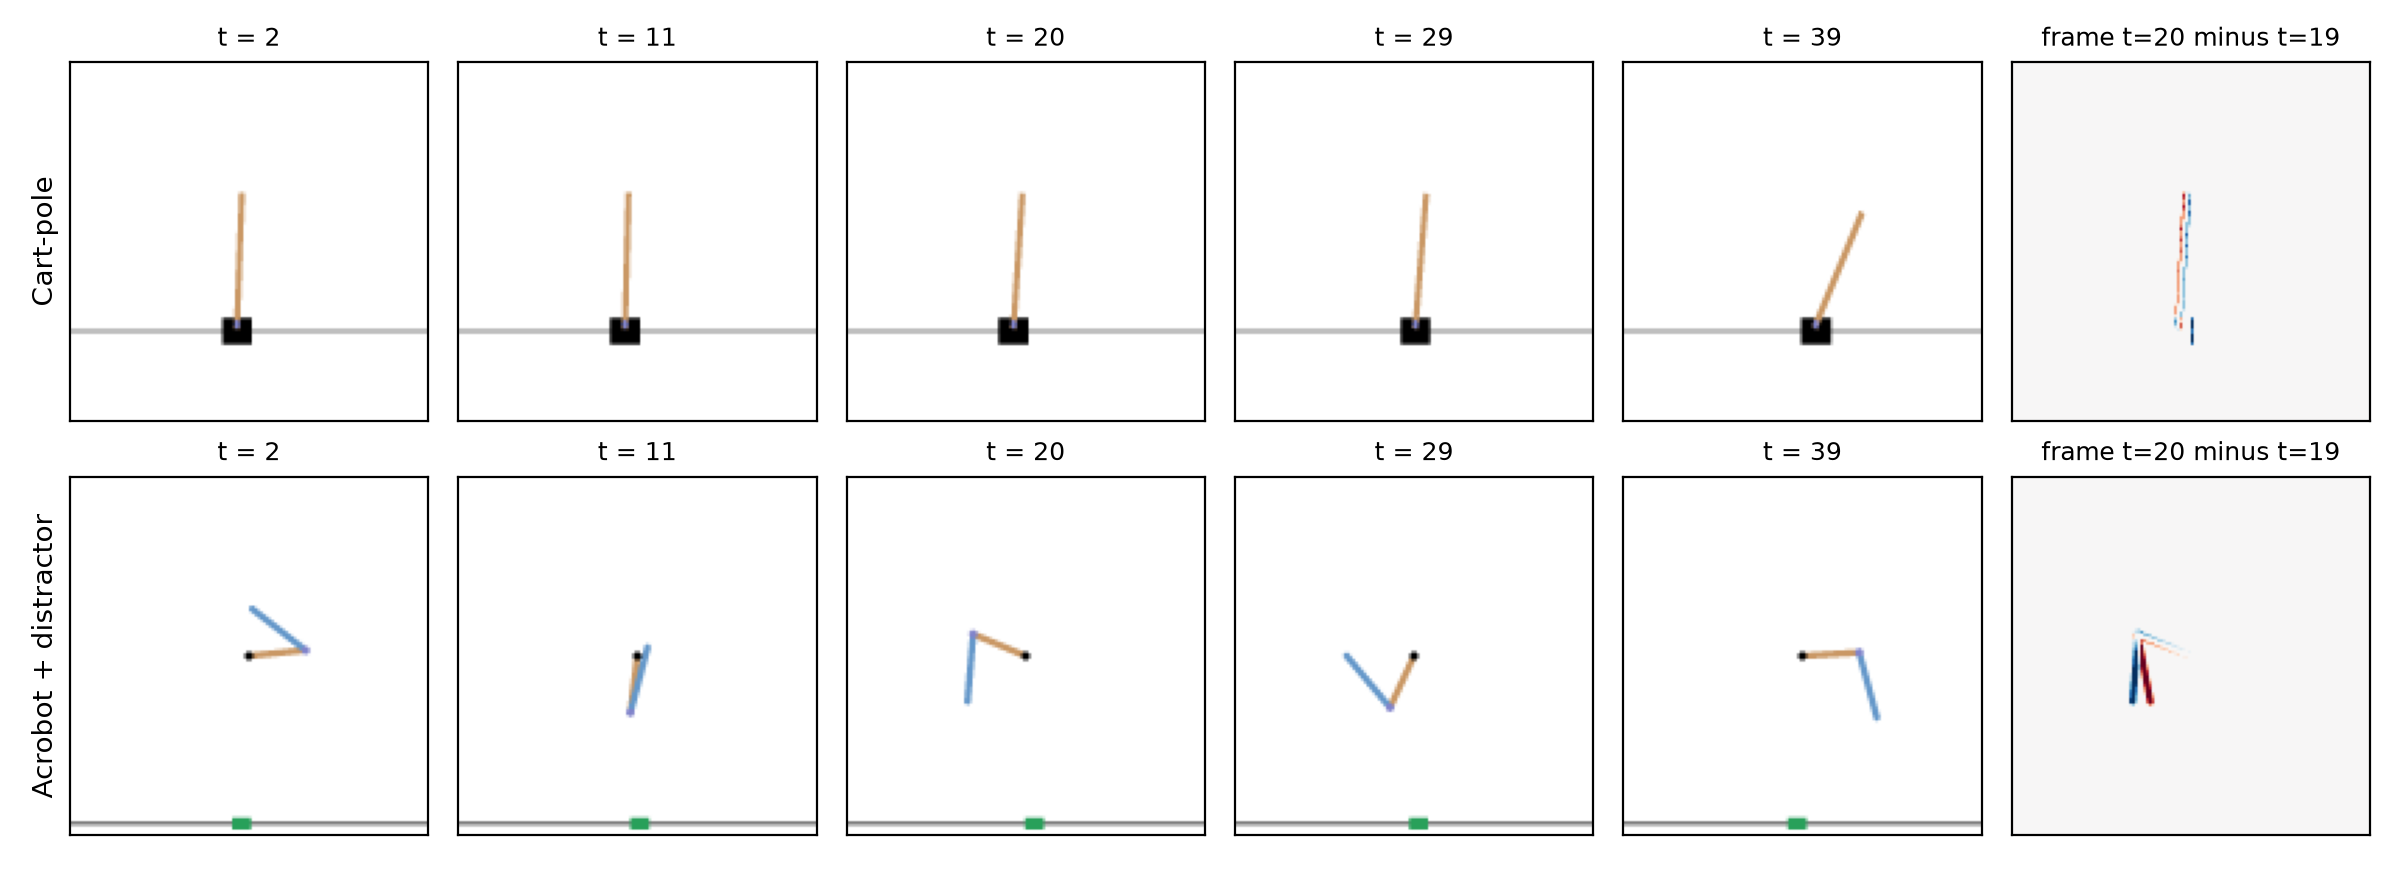
\includegraphics[width=\textwidth]{env_frames.png}
\caption{What the model sees: rendered frames from one test episode of each environment, and the frame-difference channel that the encoder also receives. In the Acrobot frames the green block on the bottom track is the distractor, which moves independently of the arm.}
\label{fig:frames}
\end{figure}

\paragraph{Frame-averaged velocities.} A single image does not show velocity. The velocity variables are therefore defined as finite differences over one transition, $\vb_t = (x_t - x_{t-1})/\Delta t$ and $\wb_t = (\theta_t - \theta_{t-1})/\Delta t$, which are observable from two consecutive frames and the previous action. Check (c) in Table~\ref{tab:checks} confirms this ($\Rsq \geq 0.996$).

\section{Expert Causal Graph}

The candidate edges run from the inputs $(d_t, u_t, u_{t-1}, u_{t-2})$ to each component of the one-step change $\dd d_t = d_{t+1} - d_t$. With four states, three actions and four targets, cart-pole has $7 \times 4 = 28$ candidate edges; Acrobot has $9 \times 6 = 54$. The previous actions appear as inputs because a frame-averaged velocity at $t$ already contains part of the action $u_{t-1}$.

For each edge the normalised effect is computed from the simulator's exact Jacobian, averaged over the dataset:
\begin{equation}
e_{ij} = \mathbb{E}\left[\,\left|\frac{\partial \dd d_j}{\partial \text{in}_i}\right|\,\right] \cdot \frac{\mathrm{sd}(\text{in}_i)}{\mathrm{sd}(\dd d_j)}.
\label{eq:effect}
\end{equation}
An edge is \emph{absent} if the Jacobian is exactly zero, \emph{strong} if $e_{ij} \geq 0.1$, and \emph{weak} otherwise. The cut 0.1 was fixed in advance. Table~\ref{tab:checks} lists the six checks the answer key passes, Table~\ref{tab:cp_expert} lists the ten strong cart-pole edges, and Figure~\ref{fig:cp_expert} draws the whole cart-pole graph.

\begin{table}[htbp]
\caption{Checks on the expert graph}
\centering
\small
\begin{tabular}{| p{6.8cm} | c | c |}
\hline
\textbf{Check} & \textbf{Cart-pole} & \textbf{Acrobot} \\
\hline
(a) Equations match the Lagrangian (max error) & $2\times10^{-14}$ & $1\times10^{-15}$ \\
\hline
(b) Energy conserved with no action (drift) & $6\times10^{-5}$ & $1\times10^{-4}$ \\
\hline
(c) Velocities observable from two frames + previous action ($\Rsq$) & 0.996 & $\approx 1$ \\
\hline
(d) Jacobian zeros match the hand-derived graph & yes & yes (22 cross edges zero) \\
\hline
(e) Strong / weak / absent edges & 10 / 7 / 11 & 20 / 8 / 26 \\
\hline
(f) History gain when physics is hidden & 0.090 & 0.098 \\
\hline
\end{tabular}
\label{tab:checks}
\end{table}

\begin{table}[htbp]
\caption{Strong edges of the cart-pole expert graph, with normalised effect $e_{ij}$}
\centering
\small
\begin{tabular}{| c | c || c | c |}
\hline
\textbf{Edge} & $e_{ij}$ & \textbf{Edge} & $e_{ij}$ \\
\hline
$\vb \rightarrow \dd x$ & 0.95 & $\theta \rightarrow \dd\theta$ & 0.15 \\
$u_{t-1} \rightarrow \dd x$ & 0.15 & $\wb \rightarrow \dd\theta$ & 0.85 \\
$\theta \rightarrow \dd\vb$ & 0.15 & $\theta \rightarrow \dd\wb$ & 0.86 \\
$u_t \rightarrow \dd\vb$ & 0.29 & $u_t \rightarrow \dd\wb$ & 0.18 \\
$u_{t-1} \rightarrow \dd\vb$ & 0.87 & $u_{t-1} \rightarrow \dd\wb$ & 0.56 \\
\hline
\end{tabular}
\label{tab:cp_expert}
\end{table}

\begin{figure}[htbp]
\centering
\begin{tikzpicture}[
    inp/.style={draw, circle, minimum size=9mm, inner sep=0pt, font=\small, fill=simc},
    out/.style={draw, rounded corners=2pt, minimum width=12mm, minimum height=8mm, font=\small, fill=modc},
    st/.style={-{Stealth[length=2mm]}, line width=#1, black!80},
    wk/.style={-{Stealth[length=1.6mm]}, dashed, gray}]
  % inputs
  \node[inp] (x)   at (0, 0)    {$x$};
  \node[inp] (v)   at (0,-1.1)  {$\bar v$};
  \node[inp] (th)  at (0,-2.2)  {$\theta$};
  \node[inp] (w)   at (0,-3.3)  {$\bar\omega$};
  \node[inp] (u0)  at (0,-4.4)  {$u_t$};
  \node[inp] (u1)  at (0,-5.5)  {$u_{t-1}$};
  \node[inp] (u2)  at (0,-6.6)  {$u_{t-2}$};
  % targets
  \node[out] (dx)  at (7,-0.8)  {$\Delta x$};
  \node[out] (dv)  at (7,-2.5)  {$\Delta \bar v$};
  \node[out] (dth) at (7,-4.2)  {$\Delta\theta$};
  \node[out] (dw)  at (7,-5.9)  {$\Delta\bar\omega$};
  % strong edges, width ~ effect size
  \draw[st=2.9pt] (v)  -- (dx);
  \draw[st=0.9pt] (u1) -- (dx);
  \draw[st=0.9pt] (th) -- (dv);
  \draw[st=1.2pt] (u0) -- (dv);
  \draw[st=2.7pt] (u1) -- (dv);
  \draw[st=0.9pt] (th) -- (dth);
  \draw[st=2.6pt] (w)  -- (dth);
  \draw[st=2.6pt] (th) -- (dw);
  \draw[st=1.0pt] (u0) -- (dw);
  \draw[st=1.9pt] (u1) -- (dw);
  % weak edges
  \draw[wk] (th) -- (dx);
  \draw[wk] (w)  -- (dx);
  \draw[wk] (w)  -- (dv);
  \draw[wk] (w)  -- (dw);
  \draw[wk] (u0) -- (dx);
  \draw[wk] (u0) -- (dth);
  \draw[wk] (u1) -- (dth);
  % legend
  \node[font=\footnotesize, align=left, anchor=north west] at (8.2,-0.3) {%
    \tikz\draw[-{Stealth[length=2mm]}, line width=1.5pt] (0,0)--(0.7,0); strong ($e \ge 0.1$),\\[-1pt]
    \quad width $\propto e$\\[2pt]
    \tikz\draw[-{Stealth[length=1.6mm]}, dashed, gray] (0,0)--(0.7,0); weak ($0 < e < 0.1$)\\[2pt]
    no arrow: absent ($e = 0$)};
  \node[font=\footnotesize\bfseries] at (0, 0.8) {inputs at $t$};
  \node[font=\footnotesize\bfseries] at (7, 0.1) {one-step change};
\end{tikzpicture}
\caption{The cart-pole expert graph: 10 strong, 7 weak and 11 absent edges out of 28. No edge leaves $x$ or $u_{t-2}$, and $\bar v$ affects only $\Delta x$.}
\label{fig:cp_expert}
\end{figure}

Check (f) measures how much a model that sees the past (and so can infer the hidden physics) can beat a memoryless model; it gives a ceiling against which the world model's use of history can be judged. The Acrobot expert graph has 20 strong edges: 14 of the 16 arm-to-arm edges, the torque edges $u_t \rightarrow \dd\wb_2$, $u_{t-1} \rightarrow \dd\wb_1$ and $u_{t-1} \rightarrow \dd\wb_2$, and the distractor's own edges $p \rightarrow \dd p$, $p \rightarrow \dd\vb_p$ and $\vb_p \rightarrow \dd p$. There are no edges from $u_{t-2}$ and none between the arm and the distractor.

\section{JEPA World Model}

Figure~\ref{fig:jepa} shows the architecture. It has four parts:
\begin{itemize}
	\item \textbf{Encoder.} The input is a 9-channel image: the previous frame $o_{t-1}$, the current frame $o_t$ and their difference $o_t - o_{t-1}$. The difference channel makes motion visible to a single forward pass. The image is cut into $8\times8$ patches (256 tokens) plus a CLS token. These pass through a Vision Transformer (ViT) with 4 layers, width 192 and 3 heads. The CLS output passes through an MLP projector (192 $\to$ 2048 with batch normalisation $\to$ 192), giving the latent $z_t \in \mathbb{R}^{192}$.
	\item \textbf{Action embedder.} An MLP maps the action context $(u_{t-1}, u_t)$ to a 192-d conditioning vector $c_t$.
	\item \textbf{Predictor.} A transformer over the last five latents $z_{t-4..t}$, with learned position embeddings. It has 6 blocks (16 heads of size 64, MLP width 2048). Every block is conditioned on $c_t$ through adaptive layer normalisation (AdaLN-zero): $c_t$ sets the shift, scale and gate of each sub-layer. An output projector of the same form as the encoder's gives $\zh_{t+1}$.
	\item \textbf{Inverse model.} An MLP (256 hidden units) that recovers the three actions between four consecutive latents.
\end{itemize}
The training loss combines three terms:
\begin{itemize}
	\item a \textbf{rollout loss}: the MSE between $\zh_{t+k}$ and the encoder's own $z_{t+k}$ for $k = 1, 2, 3$, where each prediction is appended to the history to make the next one;
	\item an \textbf{inverse-model loss}, which forces the latent to keep action-relevant information; and
	\item the \textbf{SIGReg} regulariser \cite{balestriero2025lejepa}, which pushes the distribution of $z$ towards an isotropic Gaussian and so prevents collapse. This JEPA needs no EMA target network.
\end{itemize}
All three loss weights are 1. The model never sees state labels. The same architecture and settings are used in both environments: AdamW with learning rate $10^{-4}$ (cosine schedule, 5 warm-up epochs), batch size 64, 200 epochs and 21 saved checkpoints (every 10 epochs, including the untrained epoch 0). Table~\ref{tab:training} gives the final losses.

\begin{figure}[htbp]
\centering
\resizebox{\textwidth}{!}{%
\begin{tikzpicture}[node distance=6mm and 7mm]
  % inputs
  \node[box=simc, text width=24mm] (in) {\textbf{Input}\\ $o_{t-1}$, $o_t$, $o_t-o_{t-1}$\\ $9\times128\times128$};
  % encoder
  \node[box=modc, text width=34mm, right=of in] (enc) {\textbf{Encoder}\\ patch embed $8{\times}8$ (256 + CLS)\\ ViT: 4 layers, 192-d, 3 heads\\ MLP projector 2048 + BN};
  \node[box, text width=20mm, right=of enc] (hist) {history\\ $z_{t-4},\dots,z_t$\\ ($5\times192$)};
  % predictor
  \node[box=modc, text width=36mm, right=of hist] (pred) {\textbf{Predictor}\\ 6 transformer blocks\\ 16 heads $\times$ 64, MLP 2048\\ AdaLN-zero conditioning\\ + output projector};
  \node[box, text width=14mm, right=of pred] (zh) {$\hat z_{t+1}$};
  % actions
  \node[box=simc, text width=24mm, below=11mm of hist] (act) {\textbf{Actions}\\ $(u_{t-1}, u_t)$};
  \node[box=modc, text width=26mm, at={(pred |- act)}] (aemb) {\textbf{Action MLP}\\ $\to c_t \in \mathbb{R}^{192}$};
  % target branch
  \node[box=simc, text width=24mm, above=11mm of in] (tin) {future frames\\ $o_{t+1..t+3}$};
  \node[box=modc, text width=34mm, at={(enc |- tin)}] (tenc) {same encoder};
  \node[box, text width=14mm, at={(zh |- tin)}] (tz) {$z_{t+1..t+3}$};
  % losses
  \node[box=lossc, text width=22mm, right=of zh] (lroll) {\textbf{Rollout loss}\\ MSE, 3 steps};
  \node[box=lossc, text width=22mm, below=11mm of lroll] (linv) {\textbf{Inverse model}\\ 4 latents $\to$ 3 actions};
  \node[box=lossc, text width=34mm, at={(enc |- act)}] (lsig) {\textbf{SIGReg}: push $z$\\ towards $\mathcal{N}(0, I)$};
  % arrows
  \draw[arr] (in) -- (enc);
  \draw[arr] (enc) -- node[lab, above] {$z_t$} (hist);
  \draw[arr] (hist) -- (pred);
  \draw[arr] (pred) -- (zh);
  \draw[arr] (act) -- (aemb);
  \draw[arr] (aemb) -- node[lab, right] {shift, scale, gate} (pred);
  \draw[arr] (tin) -- (tenc);
  \draw[arr] (tenc) -- (tz);
  \draw[arr] (zh) -- (lroll);
  \draw[arr] (tz) -| (lroll);
  \draw[arr] (enc) -- node[lab, right] {$z$} (lsig);
  \draw[arr] (zh.south) |- (linv.west);
  \draw[arr, dashed] (zh.north) -- ++(0,0.45) -| node[lab, above, pos=0.25] {append to history (rollout $\times 3$)} (hist.north);
\end{tikzpicture}}
\caption{Architecture of the JEPA world model. Orange blocks are trained networks, blue blocks are data and red blocks are training losses. Encoder, predictor and inverse model are trained jointly; the model never sees state labels.}
\label{fig:jepa}
\end{figure}

\begin{table}[htbp]
\caption{Training runs of the JEPA (epoch 200)}
\centering
\small
\begin{tabular}{| p{5.2cm} | c | c |}
\hline
\textbf{Run} & \textbf{Train / val loss} & \textbf{Val rollout error} \\
\hline
Cart-pole, fixed physics & 0.021 / 0.109 & 0.0031 \\
\hline
Cart-pole, varied physics (main) & 0.024 / 0.138 & 0.0072 \\
\hline
Acrobot, varied physics & 0.025 / 0.450 & 0.023 \\
\hline
\end{tabular}
\label{tab:training}
\end{table}

\paragraph{Batch-normalisation fix.} During Acrobot training the validation loss was about 15 while the training loss was 0.13. Evaluating the training data in evaluation mode also gave about 15, which isolated the cause: the running statistics of the encoder projector's batch normalisation had drifted about 5.6 standard deviations from the true statistics. The fix recomputes these statistics from 200 training batches before every evaluation and before extraction. The validation loss fell to 0.45; the weights were unaffected. Cart-pole was checked and does not need the fix.

\section{Reading the Model: the Differential Probe}

Decoding the state from $z_t$ proves little, because the untrained encoder already decodes the pole angle with $\Rsq \approx 0.95$. The probe therefore reads the \emph{predicted change} (Figure~\ref{fig:probe}):
\begin{enumerate}
	\item \textbf{Fit.} An MLP probe $Q_D$ ($192 \rightarrow 256 \rightarrow 256 \rightarrow$ targets) is trained to map the \emph{encoder's} latent change $z_{t+1} - z_t$ to the true state change $\dd d_t$. It is cross-fitted over five episode folds.
	\item \textbf{Test.} The same probe, frozen, is applied to the \emph{predictor's} latent change $\zh_{t+1} - z_t$, giving the model's predicted change $\widehat{\dd d}_t = Q_D(\zh_{t+1} - z_t)$.
\end{enumerate}
The probe never sees predictor output while fitting. It reads the predictor correctly only if the predictor moves the latent the way the real dynamics do. A target is declared \emph{testable} only if the encoder's own change is readable, $\Rsq \geq 0.5$ (fixed in advance); otherwise its edges are not interpreted.

\begin{figure}[htbp]
\centering
\begin{tikzpicture}[node distance=5mm and 8mm]
  % fit row
  \node[font=\small\bfseries, anchor=east] (fitlab) at (0,0) {1. Fit};
  \node[box=modc, text width=22mm, right=4mm of fitlab] (e1) {Encoder\\ $z_t$, $z_{t+1}$};
  \node[box, text width=22mm, right=of e1] (dz) {encoder change\\ $z_{t+1}-z_t$};
  \node[box=anac, text width=24mm, right=of dz] (q1) {\textbf{Probe $Q_D$}\\ MLP 192-256-256\\ (trained)};
  \node[box=simc, text width=22mm, right=of q1] (y1) {true change\\ $\Delta d_t$ (simulator)};
  % test row
  \node[font=\small\bfseries, anchor=east] (testlab) at (0,-2.3) {2. Test};
  \node[box=modc, text width=22mm, right=4mm of testlab] (e2) {Predictor\\ $\hat z_{t+1}$, and $z_t$};
  \node[box, text width=22mm, right=of e2] (dzh) {predicted change\\ $\hat z_{t+1}-z_t$};
  \node[box=anac, text width=24mm, right=of dzh] (q2) {\textbf{Probe $Q_D$}\\ same weights\\ (frozen)};
  \node[box=lossc, text width=22mm, right=of q2] (y2) {model's change\\ $\widehat{\Delta d}_t$ $\to$ edge tests};
  \draw[arr] (e1) -- (dz);
  \draw[arr] (dz) -- (q1);
  \draw[thick, {Stealth[length=2.2mm]}-{Stealth[length=2.2mm]}] (q1) -- node[lab, above] {loss} (y1);
  \draw[arr] (e2) -- (dzh);
  \draw[arr] (dzh) -- (q2);
  \draw[arr] (q2) -- (y2);
  \draw[arr, dashed] (q1) -- node[lab, right] {copy, freeze} (q2);
\end{tikzpicture}
\caption{The differential probe. It is fitted only on the encoder's latent changes against the true state changes, then frozen and applied to the predictor's latent changes. It reads the predictor correctly only if the predictor moves the latent the way real dynamics do.}
\label{fig:probe}
\end{figure}

\section{Edge Scoring}

For each target $j$, a masked MLP predicts $\widehat{\dd d}_{t,j}$ from the true inputs $(d_t, u_t, u_{t-1}, u_{t-2})$ plus independently shuffled \emph{decoy} copies of the inputs. For each of $S = 50$ random half-splits of the episodes, the network is fitted on one half and evaluated on the other, once with all inputs and once without input $i$. The LOCO statistic of edge $i \rightarrow j$ is the loss of accuracy when $i$ is dropped, relative to the strongest decoy. Splitting by episode, not by row, keeps correlated time steps on the same side of the split.

\section{Pruning: Null-Calibrated Max-$T$}

A rule is needed that turns the edge statistics into a kept/dropped decision. Eight rules were compared on cart-pole (Table~\ref{tab:pruning}) on four \emph{validation graphs} whose outcome does not depend on the model's quality: the graph from true data, the graph from true data with noise matched to the probe's error, a pure-noise graph (shuffled targets, should keep 0 edges) and the untrained model (should keep 0 edges). The chosen rule, \emph{null-calibrated max-$T$}, was declared before its results were seen:
\begin{enumerate}
	\item Repeat the full scoring $K = 20$ times with the target rows shuffled, and record the maximum statistic over all edges in each repeat, $T^{*}_k$.
	\item For each edge with statistic $T_{ij}$, compute the exact permutation $p$-value
	\begin{equation}
	p_{ij} = \frac{1 + \#\{k : T^{*}_k \geq T_{ij}\}}{K + 1}.
	\label{eq:maxT}
	\end{equation}
	\item Keep the edge if $p_{ij} \leq 0.05$.
\end{enumerate}
Comparing every edge with the null \emph{maximum} controls the family-wise error rate \cite{westfall1993resampling}: under the global null, the probability that the graph contains any false edge is at most 5\%. With $K = 20$ the smallest attainable $p$ is $1/21 \approx 0.048$, so an edge is kept only if it beats all 20 null maxima.

\begin{table}[htbp]
\caption{Pruning rules compared on cart-pole. Each cell: strong-graph F1 $\cdot$ edges kept $\cdot$ false positives}
\centering
\footnotesize
\begin{tabular}{| p{3.2cm} | c | c | c | c | c |}
\hline
\textbf{Rule} & \textbf{True data} & \textbf{Noise-matched} & \textbf{Noise (0)} & \textbf{Untrained (0)} & \textbf{Trained} \\
\hline
Decoy margin & .75 $\cdot$ 9 $\cdot$ 0 & .46 $\cdot$ 3 $\cdot$ 0 & 0 & 0 & .57 $\cdot$ 4 $\cdot$ 0 \\
\hline
FDR & .65 $\cdot$ 26 $\cdot$ 11 & .74 $\cdot$ 23 $\cdot$ 7 & 11 & 0 & .69 $\cdot$ 19 $\cdot$ 7 \\
\hline
Minimum effect & .84 $\cdot$ 10 $\cdot$ 1 & .84 $\cdot$ 10 $\cdot$ 1 & 7 & 0 & .75 $\cdot$ 7 $\cdot$ 0 \\
\hline
Jacobian effect & .78 $\cdot$ 15 $\cdot$ 4 & .75 $\cdot$ 16 $\cdot$ 5 & 16 & 28 & .77 $\cdot$ 19 $\cdot$ 6 \\
\hline
Effect + FDR & .78 $\cdot$ 14 $\cdot$ 4 & .75 $\cdot$ 15 $\cdot$ 5 & 11 & 0 & .72 $\cdot$ 17 $\cdot$ 6 \\
\hline
Knockoffs & .74 $\cdot$ 12 $\cdot$ 2 & 0 kept & 0 & 0 & 0 kept \\
\hline
Null-cal., per edge & .84 $\cdot$ 10 $\cdot$ 1 & .84 $\cdot$ 10 $\cdot$ 1 & 3 & 0 & .75 $\cdot$ 7 $\cdot$ 0 \\
\hline
\textbf{Null-cal., max-$T$} & \textbf{.84 $\cdot$ 10 $\cdot$ 1} & \textbf{.84 $\cdot$ 10 $\cdot$ 1} & \textbf{0} & \textbf{0} & \textbf{.75 $\cdot$ 6 $\cdot$ 0} \\
\hline
\end{tabular}
\label{tab:pruning}
\end{table}

The max-$T$ rule is the only rule that keeps no edge on pure noise and none on the untrained model while recovering the true-data graph as well as the most sensitive rules. Two refinements (a collinearity-scaled VIF rule and physics conditioning) were tried and pre-declared to be adopted only if they produced 0 false positives on the trained model; they produced 3, so max-$T$ remained the rule. For Acrobot the rule and the differential probe were fixed in advance, with no rule comparison.

\section{Evaluation Metrics}

The recovered graph is compared with the expert graph on the \emph{strong} edges (weak edges have effects below 0.1 and are out of reach of any finite-sample test). Reported metrics are the F1 score, the number of edges kept, the number of false positives (edges kept that are absent in the expert graph), and the AUROC of the edge statistic as a ranking of strong versus non-strong edges.

\section{Summary}

This chapter described the two environments and their hidden physics, the expert graph derived from the exact Jacobian and its six checks, the pixels-only JEPA, the differential probe that reads the predictor through a probe fitted on the encoder, the LOCO edge scoring with decoys, and the null-calibrated max-$T$ pruning rule selected on model-independent validation graphs.

%----------------------------------------------------------------------------------------

\chapter{Simulation Results}
\thispagestyle{empty}

\section{Introduction}

This chapter reports the recovered graphs. For each environment it gives the probe accuracy, the graph from true data (the best the method can do), the graph from the trained model at epoch 200 and the graph from the untrained model at epoch 0 (the floor). It then gives the cart-pole training curve and the Acrobot replication on unseen episodes.

\section{Cart-Pole}

\subsection{Probe accuracy}

Table~\ref{tab:cp_r2} gives the $\Rsq$ of the predictor change read through the differential probe. A model trained on fixed physics and tested on varied physics loses accuracy on the accelerations ($\dd\vb$, $\dd\wb$); in particular a heavy cart ($M$ 1.56--2 kg) gives $\Rsq = -0.04$ on $\dd\vb$. The model trained on varied physics recovers this ($\Rsq = 0.93$ for the heavy cart). Its $\dd\vb$ accuracy (0.94) exceeds the 0.89 ceiling for a model without history from check (f), so the model uses its five-latent history to infer the hidden physics. The untrained model's predictor change $\Rsq$ is strongly negative.

\begin{table}[htbp]
\caption{Cart-pole: predictor-change $\Rsq$ through the differential probe}
\centering
\small
\begin{tabular}{| p{6.2cm} | c | c | c | c |}
\hline
\textbf{Model} & $\dd x$ & $\dd\vb$ & $\dd\theta$ & $\dd\wb$ \\
\hline
Trained on fixed physics, tested on fixed & 0.95 & 0.98 & 0.87 & 0.91 \\
\hline
Trained on fixed physics, tested on varied & 0.90 & 0.65 & 0.79 & 0.66 \\
\hline
Trained on varied physics (main) & 0.85 & 0.94 & 0.90 & 0.86 \\
\hline
\end{tabular}
\label{tab:cp_r2}
\end{table}

\subsection{Recovered graph}

Table~\ref{tab:cp_graph} compares the graphs and Figure~\ref{fig:cp_graph} shows them as matrices.

\begin{table}[htbp]
\caption{Cart-pole graphs (varied physics, 50 splits, max-$T$ rule)}
\centering
\small
\begin{tabular}{| p{2.6cm} | c | p{4.4cm} | p{3.2cm} |}
\hline
\textbf{Graph} & \textbf{Kept} & \textbf{Missed strong edges} & \textbf{False positives} \\
\hline
True data & 10 & $\theta\rightarrow\dd\vb$, $\theta\rightarrow\dd\theta$ & $\vb\rightarrow\dd\wb$ \\
\hline
Trained model & 6 & $\theta\rightarrow\dd\vb$, $\theta\rightarrow\dd\theta$, $\theta\rightarrow\dd\wb$, $\wb\rightarrow\dd\theta$ & none \\
\hline
Untrained model & 0 & all & none \\
\hline
\end{tabular}
\label{tab:cp_graph}
\end{table}

\begin{figure}[htbp]
\centering
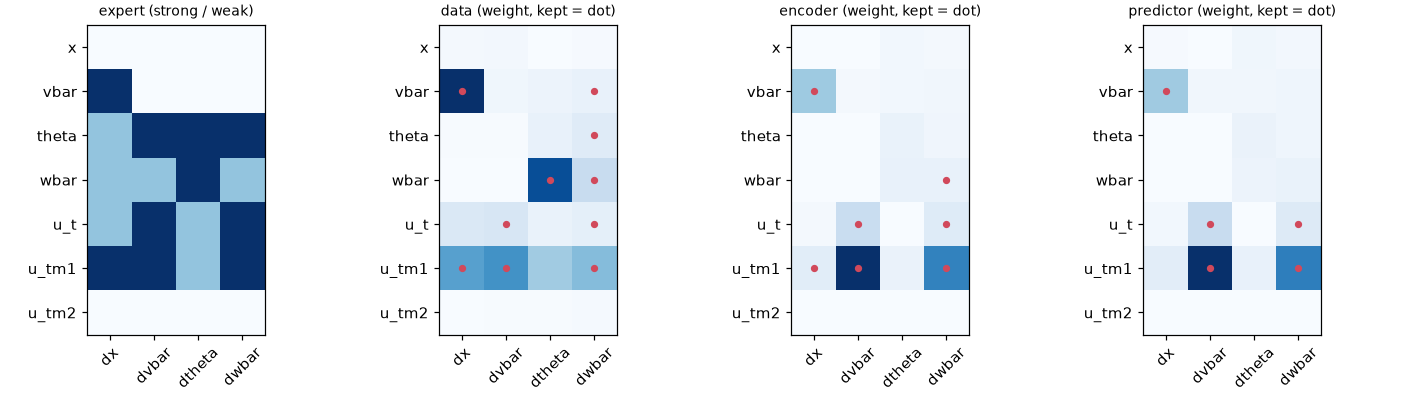
\includegraphics[width=\textwidth]{cp_graphs_e200.png}
\caption{Cart-pole graphs at epoch 200: expert graph, true-data graph, encoder graph and predictor graph. Colour is the edge weight; dots mark kept edges.}
\label{fig:cp_graph}
\end{figure}

The trained model's graph keeps $\vb \rightarrow \dd x$ and all five strong action edges, with no false positive (strong-graph F1 0.75). Three observations explain the rest:
\begin{itemize}
	\item \textbf{The pole edges are missed because of collinearity.} $\theta$ and $\wb$ are about 95--99\% predictable from the other inputs, so a leave-one-out test, which measures only unique information, sees less than 1\% of the target variance. The true-data graph misses two of the same edges, so this is a limit of the test, not only of the model.
	\item \textbf{The true-data false positive comes from hidden physics.} Conditioning the fit on each episode's $(M, m, l, g)$ removes it (effect $0.43 \rightarrow 0.04$), while conditioning on shuffled physics does not.
	\item \textbf{The encoder and predictor graphs agree closely} (Spearman 0.99), so the predictor is not the bottleneck of the graph.
\end{itemize}

\subsection{Training curve}

The predictor graph was recovered at all 21 checkpoints (20 splits, max-$T$ rule; Figure~\ref{fig:cp_curve} and Table~\ref{tab:cp_curve}).

\begin{figure}[htbp]
\centering
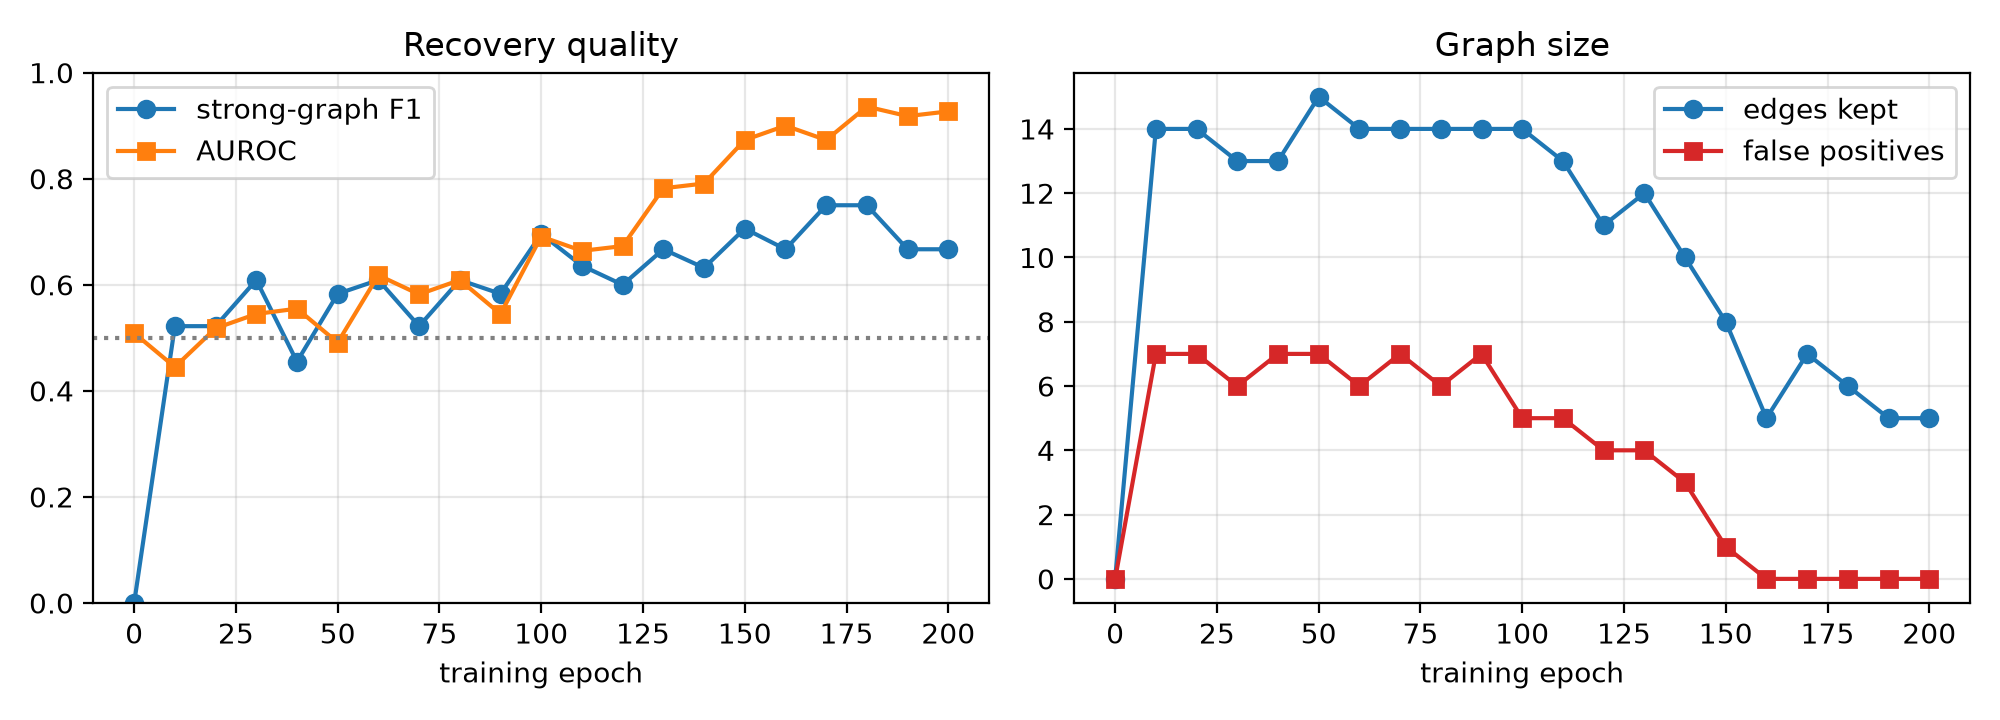
\includegraphics[width=\textwidth]{cp_curve.png}
\caption{Cart-pole: quality and size of the predictor graph across 21 training checkpoints.}
\label{fig:cp_curve}
\end{figure}

\begin{table}[htbp]
\caption{Cart-pole predictor graph by training epoch (selected checkpoints)}
\centering
\small
\begin{tabular}{| c | c | c | c | c |}
\hline
\textbf{Epoch} & \textbf{Strong F1} & \textbf{AUROC} & \textbf{Kept} & \textbf{False positives} \\
\hline
0 & 0.000 & 0.509 & 0 & 0 \\
10 & 0.522 & 0.445 & 14 & 7 \\
50 & 0.583 & 0.491 & 15 & 7 \\
100 & 0.696 & 0.691 & 14 & 5 \\
130 & 0.667 & 0.782 & 12 & 4 \\
150 & 0.706 & 0.873 & 8 & 1 \\
160 & 0.667 & 0.900 & 5 & 0 \\
180 & 0.750 & 0.936 & 6 & 0 \\
200 & 0.667 & 0.927 & 5 & 0 \\
\hline
\end{tabular}
\label{tab:cp_curve}
\end{table}

The untrained predictor keeps no edges. During epochs 10--90 the AUROC stays near chance (0.45--0.62) and the graph keeps 13--15 edges, 6--7 of them false; at this stage the predictor's change $\Rsq$ for $\dd\theta$ and $\dd\wb$ is still strongly negative ($-4.3$ and $-3.0$ at epoch 10). Between epochs 100 and 160 the AUROC rises from 0.69 to 0.90 and the false positives fall from 5 to 0. From epoch 160 on, the graph keeps 5--7 edges, all correct. The graph therefore becomes \emph{smaller and cleaner} over training. Late differences in F1 (0.75 versus 0.67) amount to one or two edges and are not a trend.

\section{Acrobot}

\subsection{True-data graph}

On true data the method recovers the Acrobot graph with strong-graph F1 0.97 and no false positive; none of the 22 arm--distractor edges is kept. It misses one strong edge and all eight weak edges.

\subsection{Probe accuracy}

\begin{table}[htbp]
\caption{Acrobot: change $\Rsq$ of the differential probe}
\centering
\small
\begin{tabular}{| c | c | c | c | c | c |}
\hline
 & \multicolumn{3}{c|}{\textbf{Trained (epoch 200)}} & \multicolumn{2}{c|}{\textbf{Untrained (epoch 0)}} \\
\hline
\textbf{Target} & Encoder & Predictor & Testable & Encoder & Predictor \\
\hline
$\dd\theta_1$ & 0.88 & 0.90 & yes & 0.25 & $-3.4$ \\
$\dd\wb_1$ & 0.77 & 0.79 & yes & 0.00 & $-2.1$ \\
$\dd\theta_2$ & 0.68 & 0.72 & yes & 0.06 & $-2.3$ \\
$\dd\wb_2$ & 0.76 & 0.79 & yes & 0.01 & $-2.3$ \\
$\dd p$ (distractor) & $-0.03$ & $-0.02$ & no & 0.75 & $-5.4$ \\
$\dd\vb_p$ (distractor) & $-0.03$ & $-0.02$ & no & $-0.06$ & $-1.2$ \\
\hline
\end{tabular}
\label{tab:ac_r2}
\end{table}

The four arm targets are readable (Table~\ref{tab:ac_r2}). The distractor is not encoded by the trained model: nothing in the training loss rewards it, and the untrained encoder in fact reads $\dd p$ better ($\Rsq$ 0.75) than the trained one ($-0.03$), so training \emph{discarded} the distractor. The model also memorises its training episodes: at epoch 150 action recovery by the inverse model is $\Rsq$ 0.99 on training episodes and $-0.38$ on new ones.

\subsection{Recovered graph}

\begin{table}[htbp]
\caption{Acrobot predictor graph (50 splits, max-$T$ rule)}
\centering
\small
\begin{tabular}{| p{6.4cm} | p{3.6cm} | p{3.4cm} |}
\hline
 & \textbf{Trained (epoch 200)} & \textbf{Untrained (epoch 0)} \\
\hline
Readable targets: F1 $\cdot$ FP $\cdot$ missed & \textbf{1.00 $\cdot$ 0 $\cdot$ 0} & 0.00 $\cdot$ 2 $\cdot$ 2 \\
\hline
All 54 edges: strong F1 $\cdot$ kept $\cdot$ FP & 0.72 $\cdot$ 29 $\cdot$ 10 & 0.17 $\cdot$ 4 $\cdot$ 2 \\
\hline
Strong-graph AUROC & 0.83 & 0.52 \\
\hline
Weak edges recovered & 2 / 8 & 0 / 8 \\
\hline
Distractor $\rightarrow$ arm edges kept (0 expected) & 0 / 8 & 0 / 8 \\
\hline
\end{tabular}
\label{tab:ac_graph}
\end{table}

\begin{figure}[htbp]
\centering
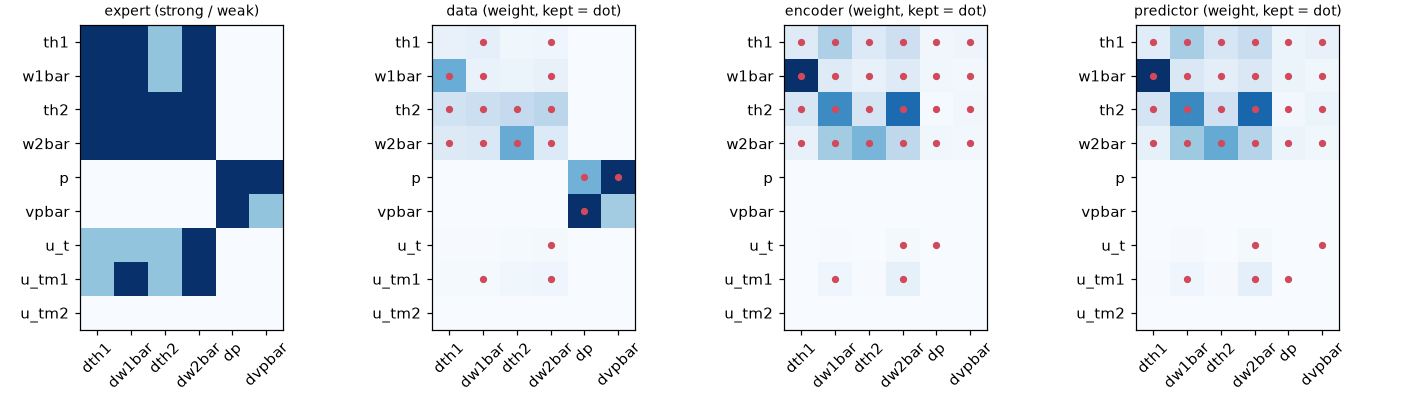
\includegraphics[width=\textwidth]{ac_graphs_e200.png}
\caption{Acrobot graphs at epoch 200: expert (dark = strong, light = weak), true data, encoder and predictor. Dots mark kept edges.}
\label{fig:ac_graph}
\end{figure}

On the four readable targets the trained model's graph matches the expert graph \emph{exactly}: all 17 strong edges and all 12 absent edges into those targets are correct, including every angle edge (Table~\ref{tab:ac_graph}, Figure~\ref{fig:ac_graph}). The encoder's own graph is identical on these targets. The ten false positives of the full graph all point into the two unreadable distractor targets ($\dd p$, $\dd\vb_p$): the probe's output for those targets is noise that varies with the arm, so these edges say nothing about the model and should be excluded by the testability rule. No edge from the distractor into the arm is kept. Unlike cart-pole, the untrained predictor's floor is not empty: it keeps four edges, two of them false. The model also responds slightly to $u_{t-2}$ (effect 0.05--0.08) where the truth is exactly zero, but no $u_{t-2}$ edge is kept.

\subsection{Replication on unseen episodes}

Because the Acrobot model memorises, the graph was recomputed on 190 validation episodes that the model never trained on (6,310 rows, eight times fewer than training), with the probe, the null and the scoring redone at this size. The true-data graph at this size is perfect (F1 1.00), so the sample is large enough.

\begin{table}[htbp]
\caption{Acrobot predictor graph on training versus unseen episodes}
\centering
\small
\begin{tabular}{| p{6.2cm} | p{3.4cm} | p{3.4cm} |}
\hline
 & \textbf{Training episodes} & \textbf{Unseen episodes} \\
\hline
All 54 edges: strong F1 & 0.72 & 0.74 \\
\hline
Strong-graph AUROC & 0.83 & 0.84 \\
\hline
Kept $\cdot$ false positives $\cdot$ missed & 29 $\cdot$ 10 $\cdot$ 3 & 26 $\cdot$ 7 $\cdot$ 4 \\
\hline
Readable targets: F1 $\cdot$ FP $\cdot$ missed & 1.00 $\cdot$ 0 $\cdot$ 0 (4 targets) & 0.97 $\cdot$ 0 $\cdot$ 1 (3 targets) \\
\hline
Probe $\Rsq$: $\dd\theta_1$, $\dd\wb_1$, $\dd\theta_2$, $\dd\wb_2$ & .90, .79, .72, .79 & .79, .56, .51, .60 \\
\hline
\end{tabular}
\label{tab:ac_val}
\end{table}

The graph holds on unseen episodes (Table~\ref{tab:ac_val}): overall quality is unchanged, readable targets give no false positive, and the single miss is the borderline strong edge $u_t \rightarrow \dd\wb_2$ (effect 0.118). Only three targets count as readable here, because $\dd\theta_2$ falls just under the cut ($\Rsq$ 0.49). The read-out is weaker on unseen episodes, but the probe was refitted on about a fifth as many rows, so this mixes generalisation with probe sample size. \emph{Memorisation does not break the recovered graph.}

\section{Summary}

This chapter presented the simulation results. On cart-pole the trained model's graph contains only true edges but misses the collinear pole-angle edges; over training it shrinks from 14 edges with 7 false to 5 correct edges. On Acrobot the model's graph matches the expert exactly on the readable targets, on both training and unseen episodes, while the distractor, which the model discards, produces untestable targets. In both environments the untrained model gives no comparable graph, so the recovered structure is learned.

%----------------------------------------------------------------------------------------

\chapter{Counterfactual Evaluation and Graph Priors}
\thispagestyle{empty}

\section{Counterfactual Evaluation}

\subsection{Objective}

Edge agreement with the expert leaves three questions open: does the recovered graph describe the \emph{model}; when the recovered graph and the expert disagree, is it a model error or a discovery error; and do the graphs give the right \emph{effects}, not just the right edges? A counterfactual query answers all three. For one real window of a test episode it asks: had input $i$ been different, with everything else at time $t$ held fixed, what would the next change have been? The query is put to every source that can answer it and the answers are compared window by window.

\subsection{Method}

\paragraph{Interventions with a consistent history.} The model must be given frames, not states. Changing a state at $t$ directly would put a jump in the five-frame history. Instead the start state $s_{t-5}$ is solved for (vectorised damped Newton, residual below $10^{-11}$ sd), so that simulating the window forward with the episode physics and the counterfactual actions reaches the intervened state exactly at $t$ (Figure~\ref{fig:cf_resolve}). The whole window is then re-simulated and re-rendered. Each intervention has size $\delta = \kappa \cdot \mathrm{sd}(\text{input})$ with $\kappa = 0.25$ (main) and $0.5$ (sensitivity), applied with both signs. Interventions are made on every state, every action and every hidden physics parameter, on at most 3000 windows from the test split, which no earlier analysis used.

\begin{figure}[htbp]
\centering
\begin{tikzpicture}[st/.style={draw, circle, minimum size=10mm, inner sep=0pt, font=\scriptsize, fill=simc}]
  \foreach \i/\lbl in {0/{t-5}, 1/{t-4}, 2/{t-3}, 3/{t-2}, 4/{t-1}} {
    \node[st] (s\i) at (1.6*\i, 0) {$s_{\lbl}$};
  }
  \node[st, fill=lossc, very thick] (s5) at (8.0, 0) {$s'_t$};
  \node[st] (s6) at (9.6, 0) {$s'_{t+1}$};
  \foreach \a/\b in {0/1, 1/2, 2/3, 3/4, 4/5, 5/6} { \draw[arr] (s\a) -- (s\b); }
  \node[lab, align=center, below=2mm of s0] {solved for\\ (Newton)};
  \node[lab, align=center, below=2mm of s5] {$d_i(t) \to d_i(t) + \delta$\\ others held fixed};
  \node[lab, align=center, above=2mm of s3] {re-simulated with episode physics and counterfactual actions};
  \draw[decorate, decoration={brace, amplitude=5pt, mirror}] ($(s0.south west)+(0,-1.0)$) -- ($(s6.south east)+(0,-1.0)$)
     node[midway, below=6pt, font=\footnotesize, align=center] {7 frames re-rendered $\to$ JEPA (model and ceiling) \quad and \quad simulator (truth)};
\end{tikzpicture}
\caption{Counterfactual intervention with a consistent history. Instead of editing the state at $t$, which would put a jump in the model's five-frame history, the start of the window is solved so that the simulator reaches the intervened state exactly at $t$.}
\label{fig:cf_resolve}
\end{figure}

\paragraph{Sources.} Each query is answered by: the \emph{truth} (simulator); the \emph{ceiling} (the encoder on the true counterfactual frames, read by the probe, i.e. the best the read-out can do); the \emph{model} (the JEPA predictor on the counterfactual history, read by the probe); an \emph{expert-graph SCM} (one masked MLP per target using only expert parents, fitted on true changes); and a \emph{recovered-graph SCM} (the same with the recovered parents, fitted on the model's read-out changes).

\paragraph{Metrics.} The per-window effect $e = \mathrm{sign}\cdot(\text{change}' - \text{change})/(\kappa\cdot \mathrm{sd}(\text{target}))$ is in the same unit as the expert effect sizes (Eq.~\ref{eq:effect}). The counterfactual effect (CE) is the mean $|e|$ over windows with a 95\% episode-bootstrap interval; CF-$\Rsq$ measures window-by-window agreement. A \emph{readout floor} is the largest upper 95\% bound of the ceiling CE over cells whose true effect is exactly zero; a cell whose model CE lower bound exceeds the floor is an edge the model demonstrably uses. The recovered graph is then scored against this \emph{model-interventional graph}.

\paragraph{Sanity checks (pre-declared).} In both environments the truth CE on expert-absent cells is at most $1.1 \times 10^{-12}$ and the Spearman correlation between the truth CE and the expert effect sizes is at least 0.992: both checks pass. The counterfactual frames are bit-identical to the simulator's renderer. One pre-declared check failed for Acrobot: the re-rendered factual frames differ from the stored frames by up to 9 pixel levels instead of the planned 2 (mean $5.5 \times 10^{-7}$). The likely cause is float32 storage of the states and is not yet confirmed. Every effect is measured against the re-rendered factual, so the offset cancels, but the check is reported as failed.

\subsection{Results}

\begin{figure}[htbp]
\centering
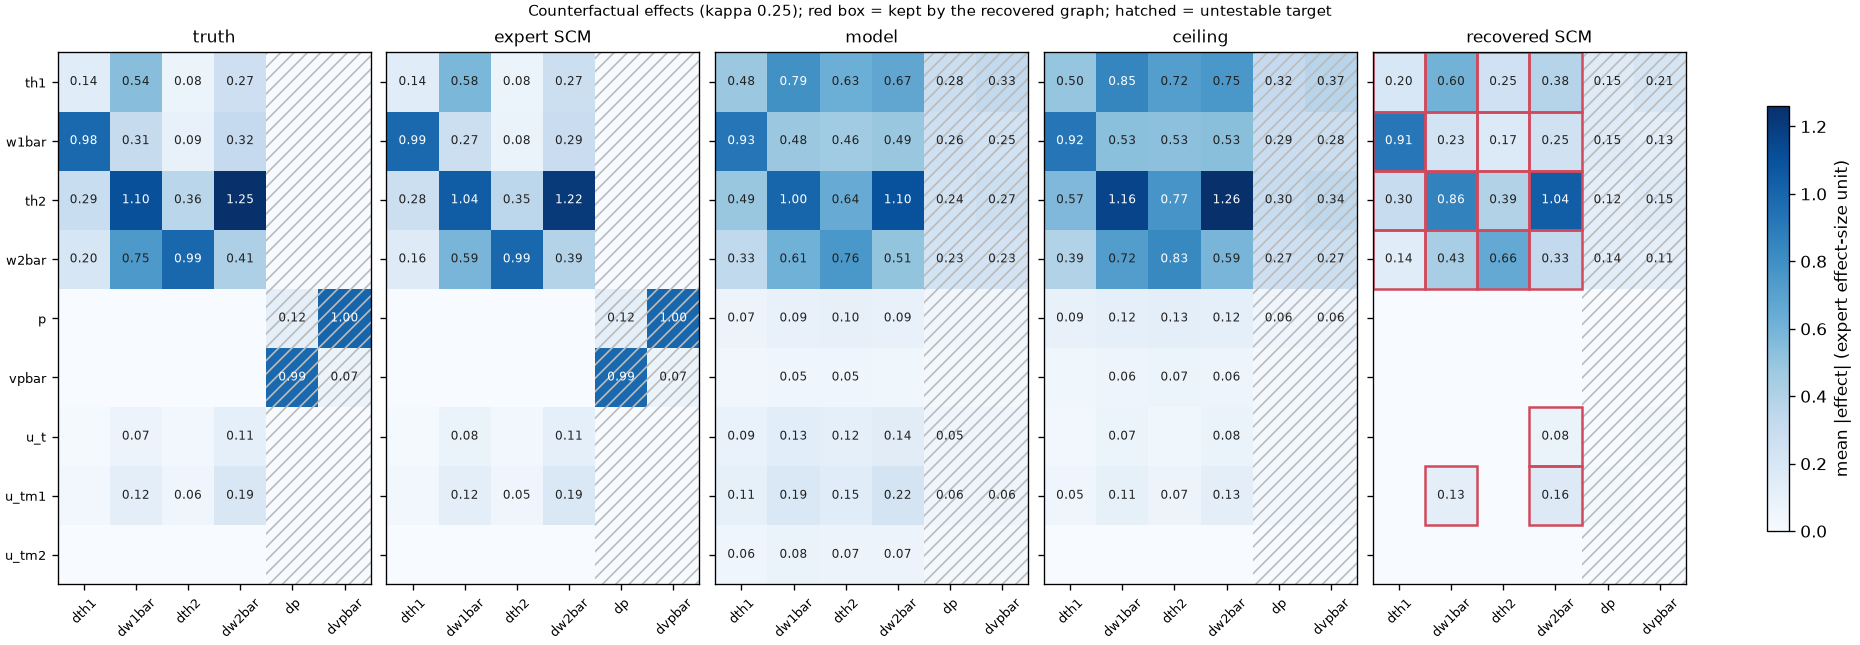
\includegraphics[width=\textwidth]{ac_cf_heatmaps.png}
\caption{Acrobot counterfactual effects ($\kappa = 0.25$) for each source. Red boxes mark edges kept by the recovered graph; hatched columns are untestable targets.}
\label{fig:ac_cf}
\end{figure}

\begin{table}[htbp]
\caption{Counterfactual agreement at epoch 200 ($\kappa = 0.25$; in brackets $\kappa = 0.5$)}
\centering
\small
\begin{tabular}{| p{7.2cm} | c | c |}
\hline
\textbf{Quantity} & \textbf{Cart-pole} & \textbf{Acrobot} \\
\hline
Readout floor & 0.634 (0.339) & 0.135 (0.076) \\
\hline
CE Spearman, model vs truth & 0.23 (0.31) & 0.93 (0.96) \\
\hline
CE Spearman, recovered SCM vs model & 0.24 (0.29) & 0.94 (0.94) \\
\hline
Recovered vs model-interventional graph, F1 & 0.44 (0.50) & \textbf{0.95} (0.88) \\
\hline
Model-interventional vs expert graph, F1 (FP) & 0.30 (0.52), 0 FP & 0.88 (1.00), 0 FP \\
\hline
\end{tabular}
\label{tab:cf}
\end{table}

\paragraph{Acrobot.} The read-out is sharp enough for the test to be informative (floor 0.135). The model's effects rank like the true effects (CE Spearman 0.93), and the recovered graph matches the graph of inputs the model demonstrably uses with F1 0.95 (18 agreeing edges, one false alarm, one miss; Figure~\ref{fig:ac_cf}, Table~\ref{tab:cf}). The model-interventional graph has no false positive against the expert, and at $\kappa = 0.5$ it equals the expert graph exactly. So on Acrobot the recovered graph is a faithful description of the model, and the model's causal structure is right. Window-by-window agreement is weaker (CF-$\Rsq$ of the model against the truth is $-0.03$ at $\kappa = 0.25$ and 0.28 at $\kappa = 0.5$): the model gets the \emph{structure} and average sizes right, but not the exact effect in every state.

\paragraph{Cart-pole.} The test is \emph{not} informative for cart-pole. Even the ceiling, the encoder applied to the true counterfactual frames, shows effects of 0.36--0.57 on cells whose true effect is zero, so the readout floor is 0.634 and only three cells clear it. The probe, fitted on natural data where $\theta$, $\wb$ and $\vb$ are strongly correlated, cannot separate single-variable interventions. Cart-pole's agreement numbers therefore measure the read-out, not the model or the discovery, and are not interpreted further. Two cart-pole findings do not depend on the floor:
\begin{itemize}
	\item \textbf{Hidden-physics confounding is confirmed interventionally.} An all-input fit on true data with physics hidden shows large spurious effects, for example $\vb \rightarrow \dd\wb$ 0.42 and $\wb \rightarrow \dd\wb$ 1.15, where the interventional truth is 0 and 0.09. Giving the fit the physics removes them (0.03 and 0.08).
	\item \textbf{Action effects with and without a consistent history agree}: the model's CE for $u_{t-1} \rightarrow \dd\vb$ is 0.77 with the history re-solved and 0.86 with the history latents held fixed, against a truth of 0.88.
\end{itemize}

\paragraph{Multi-step rollouts.} The effects of $do(u_t)$ and $do(u_{t-1})$ were followed for 1--3 steps through autoregressive latent rollouts. Mean effect sizes track the truth at every horizon (cart-pole $do(u_{t-1})$, $\dd\vb$: truth 0.83, 0.48, 0.36; model 0.72, 0.41, 0.32 at $k = 1, 2, 3$), but window-level CF-$\Rsq$ stays negative, consistent with the one-step results.

\section{Training with the Expert Graph as a Prior}

\subsection{Objective and design}

The main study asks whether the JEPA learns the graph. This study reverses the question: the expert graph is \emph{given} to the cart-pole JEPA during training, and the run is compared with a standard JEPA on speed, generalisation and open-loop rollouts. Three arms of 100 epochs each (seed 42) were run:
\begin{itemize}
	\item \textbf{Standard}: the unchanged JEPA.
	\item \textbf{Masked}: the 192-d latent is split into slots $[x\,|\,\vb\,|\,\theta\,|\,\wb\,|\,\text{ctx}]$ (four 40-d slots and a 32-d context slot meant for the hidden physics), and the predictor's attention is masked so that each slot reads only its expert parents, itself and ctx.
	\item \textbf{Jacobian}: the predictor is unchanged, and a finite-difference penalty on $\partial\zh_j/\partial z_i$ is added for every absent edge $i \rightarrow j$.
\end{itemize}

\subsection{Results}

\begin{figure}[htbp]
\centering
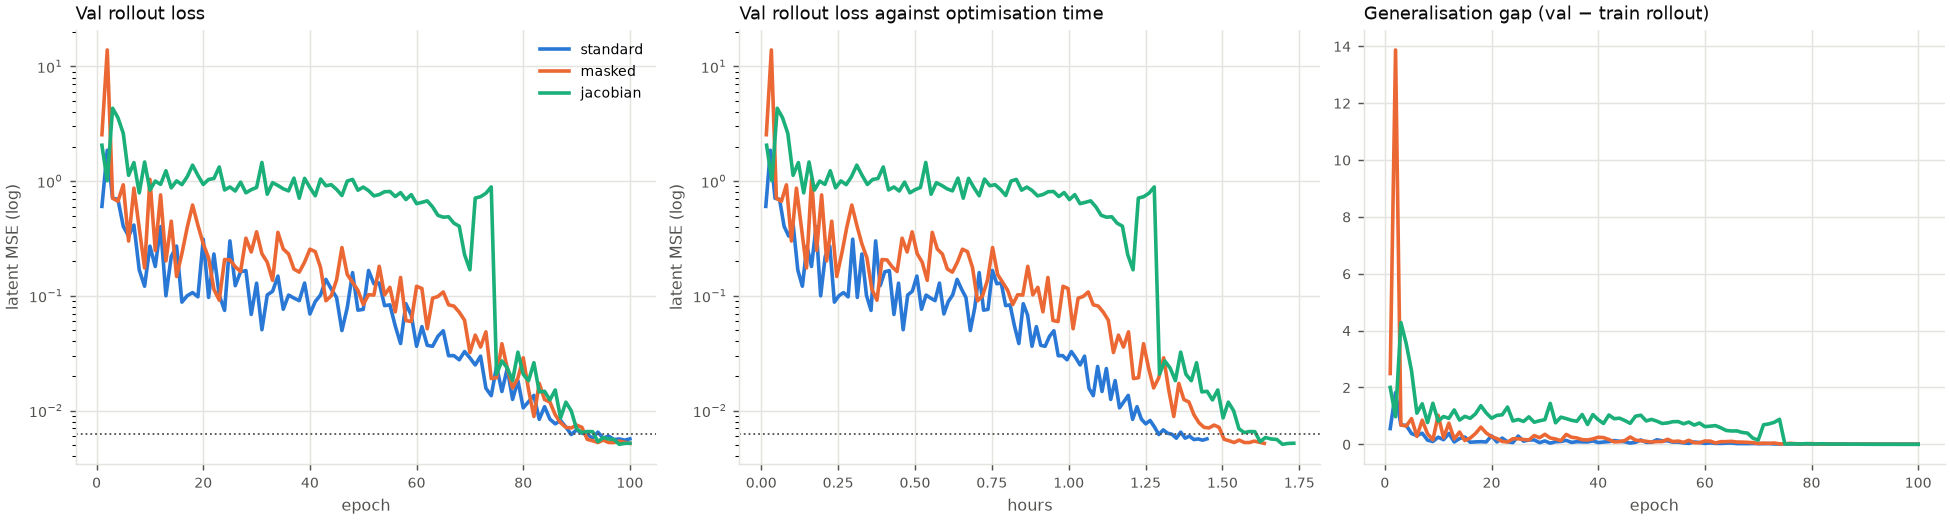
\includegraphics[width=\textwidth]{gp_training.png}
\caption{Graph-prior training: validation rollout loss against epoch and against optimisation time, and the generalisation gap.}
\label{fig:gp}
\end{figure}

\begin{table}[htbp]
\caption{Graph-prior training comparison (cart-pole, 100 epochs, one seed)}
\centering
\small
\begin{tabular}{| p{1.8cm} | p{1.4cm} | p{1.9cm} | p{2.0cm} | p{2.2cm} | p{1.9cm} |}
\hline
\textbf{Arm} & \textbf{s / epoch} & \textbf{Epochs to target} & \textbf{Final val rollout} & \textbf{Epoch $\theta$ $\Rsq \geq 0.9$} & \textbf{20-step nRMSE} \\
\hline
Standard & 52 & 89 & 0.0057 & 25 & 5.38 \\
\hline
Masked & 59 & 92 & 0.0052 & 20 & 5.38 \\
\hline
Jacobian & 62 & 94 & 0.0052 & 15 & 5.65 \\
\hline
\end{tabular}
\label{tab:gp}
\end{table}

The target is 1.1 times the standard run's final validation rollout loss. Both graph arms end with a slightly lower validation rollout loss (0.0052 versus 0.0057) and reach a pole-angle read-out of $\Rsq \geq 0.9$ earlier (epochs 20 and 15 versus 25), but they take more epochs and more wall-clock time to reach the target, and their 20-step open-loop rollouts are no better (Table~\ref{tab:gp}, Figure~\ref{fig:gp}). The Jacobian arm stays at a high loss for 70 epochs before dropping. With one seed per arm these differences are within run-to-run variation, so \emph{the graph prior gave no clear benefit}. Only five absent state edges exist in cart-pole, so a small in-distribution effect was expected.

\section{Summary}

Counterfactual queries on re-rendered interventions confirm on Acrobot that the recovered graph describes the inputs the model actually uses (F1 0.95), and that the model's interventional graph has no false edge. On cart-pole the probe cannot isolate single-variable interventions, so the counterfactual test is uninformative there, though it confirms interventionally that the true-data false positives come from hidden-physics confounding. Supplying the expert graph as a prior during training did not clearly improve the JEPA.

%----------------------------------------------------------------------------------------

\chapter{Conclusions and Future Work}
\thispagestyle{empty}
\section{Conclusions}

\begin{enumerate}
	\item A pixels-only JEPA world model does learn causal structure that can be read out of its \emph{predictions}. On Acrobot the recovered graph matches the expert graph exactly on every readable target, on training and unseen episodes, and counterfactual interventions confirm that it describes what the model uses. On cart-pole every recovered edge is true.
	\item The structure is learned, not inherited from the architecture: untrained models give an empty (cart-pole) or near-empty and wrong (Acrobot) graph, and the cart-pole graph sharpens steadily during training, from 14 edges with 7 false at epoch 10 to 5 correct edges at epoch 200.
	\item The method's limits are identifiable and were found before being mistaken for model failures: the pole-angle edges are missed because $\theta$ and $\wb$ are collinear, the true-data false positives come from hidden-physics confounding, and edges into unreadable targets carry no information.
	\item Careful controls changed the conclusions several times: the untrained-encoder control showed that state decoding proves nothing, the validation graphs rejected five sensitive pruning rules that kept edges on pure noise, and the readout floor showed that cart-pole counterfactuals are uninformative.
	\item The model can use its history to infer hidden physics ($\dd\vb$ accuracy 0.94 above the memoryless ceiling 0.89), and it discards information, such as the distractor, that its training loss does not reward.
\end{enumerate}

\section{Limitations}

\begin{itemize}
	\item The 5\% family-wise guarantee of the max-$T$ rule holds under the global null, not edge by edge when real edges are present; 20 null repeats give a coarse smallest $p$ of 0.048; and rows are shuffled across autocorrelated time steps.
	\item $\theta$ and $\wb$ are not separately identifiable by LOCO; weak edges are out of reach.
	\item The expert graph assumes known physics, while the model and the data average over it.
	\item One training seed per environment; one-step read-out for the graph.
	\item The counterfactual read-out is too coarse for cart-pole, and one pre-declared rendering check failed for Acrobot.
\end{itemize}

\section{Future scope of work}

\begin{itemize}
	\item \textbf{A second world model.} DreamerV3 has been ported to PyTorch and is being trained on the same datasets (at the time of writing about epoch 250 of 500 for cart-pole and 225 of 500 for Acrobot), so that its graph can be scored against the same expert graphs.
	\item \textbf{Stronger statistics:} 99 or more null repeats, episode-level permutations, group LOCO for the $\{\theta, \wb\}$ block, and conditional or knockoff decoys.
	\item \textbf{A sharper counterfactual read-out} for cart-pole, for example a probe trained on interventional data, and interchange interventions on the latent.
	\item \textbf{More seeds} for the main models and for the graph-prior arms, a per-output graph mask, and an Acrobot training curve.
\end{itemize}

%----------------------------------------------------------------------------------------

\newpage
\addcontentsline{toc}{chapter}{Appendix}
\appendix
\chapter{Settings and Definitions}
\thispagestyle{empty}

\section{Fixed design choices}

\begin{table}[htbp]
\caption{Settings fixed before any result}
\centering
\small
\begin{tabular}{| p{6.0cm} | p{7.6cm} |}
\hline
\textbf{Setting} & \textbf{Value} \\
\hline
Frame skip / transition & 2 / 0.04 s \\
\hline
Image size & $128 \times 128$, anti-aliased \\
\hline
Predictor history / action context & 5 latents / $(u_{t-1}, u_t)$ \\
\hline
Latent dimension & 192 \\
\hline
Encoder & 9-channel input, patch $8\times8$, ViT 4 layers $\times$ 192, 3 heads, MLP projector 2048 + BN \\
\hline
Predictor & 6 AdaLN-zero blocks, 16 heads $\times$ 64, MLP 2048, dropout 0.1 \\
\hline
Inverse model & MLP, 256 hidden, 4 latents $\to$ 3 actions \\
\hline
Losses & rollout (3 steps) + inverse + SIGReg, all weight 1 \\
\hline
Optimiser & AdamW, lr $10^{-4}$, weight decay $10^{-3}$, 5 warm-up epochs, cosine to $10^{-6}$, batch 64 \\
\hline
Training & 200 epochs, 21 checkpoints \\
\hline
Edge inputs & True simulator states \\
\hline
Probe & MLP $192 \rightarrow 256 \rightarrow 256$, 5 episode folds \\
\hline
Testable target & Encoder-change $\Rsq \geq 0.5$ \\
\hline
Strong / weak cut & Normalised effect 0.1 \\
\hline
Episode half-splits & 50 (20 for the training curve) \\
\hline
Null repeats & $K = 20$ shuffled-target repeats \\
\hline
Pruning rule & Null-calibrated max-$T$, $p \leq 0.05$ \\
\hline
Counterfactuals & Test split, $\leq 3000$ windows, $\kappa \in \{0.25, 0.5\}$, 1000 bootstrap resamples, 3 SCM seeds \\
\hline
\end{tabular}
\label{tab:settings}
\end{table}

\section{Pruning rules compared}

\begin{itemize}
	\item \textbf{Decoy margin}: keep an edge if its LOCO statistic beats the strongest decoy by $\log 1.5$ in at least 70\% of the splits.
	\item \textbf{FDR}: Benjamini--Hochberg \cite{benjamini1995fdr} on per-edge split-level $p$-values.
	\item \textbf{Minimum effect}: keep an edge whose LOCO gain exceeds a minimum effect size.
	\item \textbf{Jacobian effect}: keep an edge whose fitted Jacobian effect is at least 0.1 in the expert's unit.
	\item \textbf{Effect + FDR}: both of the above.
	\item \textbf{Knockoffs}: model-X knockoffs \cite{candes2018panning} as decoys.
	\item \textbf{Null-calibrated, per edge}: compare each edge with its own null distribution over 20 shuffled-target repeats.
	\item \textbf{Null-calibrated, max-$T$}: compare each edge with the null maximum over all edges (Eq.~\ref{eq:maxT}).
\end{itemize}

\section{Software}

All code is written in Python with PyTorch and runs on a single GPU. The simulator, renderer, JEPA, probe, edge scorer, null calibration and counterfactual engine are implemented in the project repository; the run order is documented in its README.

%----------------------------------------------------------------------------------------

\newpage
\addcontentsline{toc}{chapter}{References}
\begin{thebibliography}{99}

\bibitem{ha2018world}
D. Ha and J. Schmidhuber, ``Recurrent world models facilitate policy evolution,'' in \emph{Advances in Neural Information Processing Systems (NeurIPS)}, 2018.

\bibitem{lecun2022path}
Y. LeCun, ``A path towards autonomous machine intelligence,'' OpenReview preprint, version 0.9.2, 2022.

\bibitem{hafner2025dreamerv3}
D. Hafner, J. Pasukonis, J. Ba, and T. Lillicrap, ``Mastering diverse control tasks through world models,'' \emph{Nature}, vol. 640, pp. 647--653, 2025.

\bibitem{assran2023ijepa}
M. Assran \emph{et al.}, ``Self-supervised learning from images with a joint-embedding predictive architecture,'' in \emph{Proc. IEEE/CVF Conf. Computer Vision and Pattern Recognition (CVPR)}, 2023.

\bibitem{balestriero2025lejepa}
R. Balestriero and Y. LeCun, ``LeJEPA: Provable and scalable self-supervised learning without the heuristics,'' arXiv:2511.08544 (preprint), 2025.

\bibitem{lewm2026}
``LeWorldModel,'' arXiv:2603.19312 (preprint), 2026.

\bibitem{richens2024robust}
J. Richens and T. Everitt, ``Robust agents learn causal world models,'' in \emph{International Conference on Learning Representations (ICLR)}, 2024.

\bibitem{li2023othello}
K. Li, A. K. Hopkins, D. Bau, F. Vi\'egas, H. Pfister, and M. Wattenberg, ``Emergent world representations: Exploring a sequence model trained on a synthetic task,'' in \emph{ICLR}, 2023.

\bibitem{garrido2025intuitive}
Q. Garrido \emph{et al.}, ``Intuitive physics understanding emerges from self-supervised pretraining on natural videos,'' arXiv:2502.11831, 2025.

\bibitem{joseph2026interpreting}
Joseph \emph{et al.}, ``Interpreting physics in video world models,'' in \emph{International Conference on Machine Learning (ICML)}, 2026. arXiv:2602.07050.

\bibitem{vafa2025foundation}
K. Vafa \emph{et al.}, ``What has a foundation model found? Using inductive bias to probe for world models,'' in \emph{ICML}, 2025. arXiv:2507.06952.

\bibitem{hewitt2019control}
J. Hewitt and P. Liang, ``Designing and interpreting probes with control tasks,'' in \emph{Proc. Conf. Empirical Methods in Natural Language Processing (EMNLP)}, 2019.

\bibitem{zhang2018language}
K. Zhang and S. Bowman, ``Language modeling teaches you more than translation does: Lessons learned through auxiliary syntactic task analysis,'' in \emph{Proc. BlackboxNLP Workshop}, 2018.

\bibitem{tan2026latent}
Tan \emph{et al.}, ``What can latent world models know? Physical information in multimodal predictive representations,'' arXiv:2607.27017 (preprint), 2026.

\bibitem{zhang2026deltajepa}
Zhang, Wang \emph{et al.}, ``Delta-JEPA,'' arXiv:2606.31232 (preprint), 2026.

\bibitem{bao2026correcting}
Bao, ``Correcting a learned physical invariant improves world-model rollouts,'' arXiv:2608.23526 (preprint), 2026.

\bibitem{gonzalez2026limits}
Gonzalez Laiz and Schneider, ``Understanding the limits of latent world models,'' arXiv:2610.37588 (preprint), 2026.

\bibitem{pandaram2025sparsity}
Pandaram \emph{et al.}, ``Dynamic sparsity: Challenging common sparsity assumptions for learning world models in robotic RL benchmarks,'' arXiv:2511.08086 (preprint), 2025.

\bibitem{pearl2009causality}
J. Pearl, \emph{Causality: Models, Reasoning, and Inference}, 2nd ed. Cambridge University Press, 2009.

\bibitem{wang2022cdl}
Z. Wang, X. Xiao, Z. Xu, Y. Zhu, and P. Stone, ``Causal dynamics learning for task-independent state abstraction,'' in \emph{ICML}, 2022.

\bibitem{seitzer2021cai}
M. Seitzer, B. Sch\"olkopf, and G. Martius, ``Causal influence detection for improving efficiency in reinforcement learning,'' in \emph{NeurIPS}, 2021.

\bibitem{yao2022tdrl}
W. Yao, G. Chen, and K. Zhang, ``Temporally disentangled representation learning,'' in \emph{NeurIPS}, 2022.

\bibitem{lachapelle2022disentanglement}
S. Lachapelle \emph{et al.}, ``Disentanglement via mechanism sparsity regularization: A new principle for nonlinear ICA,'' in \emph{Conference on Causal Learning and Reasoning (CLeaR)}, 2022.

\bibitem{geiger2025causal}
A. Geiger \emph{et al.}, ``Causal abstraction: A theoretical foundation for mechanistic interpretability,'' \emph{Journal of Machine Learning Research}, 2025.

\bibitem{sutter2025nonlinear}
D. Sutter \emph{et al.}, ``The non-linear representation dilemma: Is causal abstraction enough for mechanistic interpretability?'' in \emph{NeurIPS}, 2025. arXiv:2507.08802.

\bibitem{lei2018loco}
J. Lei, M. G'Sell, A. Rinaldo, R. J. Tibshirani, and L. Wasserman, ``Distribution-free predictive inference for regression,'' \emph{Journal of the American Statistical Association}, vol. 113, no. 523, pp. 1094--1111, 2018.

\bibitem{verdinelli2024decorrelated}
I. Verdinelli and L. Wasserman, ``Decorrelated variable importance,'' \emph{Journal of Machine Learning Research}, vol. 25, 2024.

\bibitem{benjamini1995fdr}
Y. Benjamini and Y. Hochberg, ``Controlling the false discovery rate: A practical and powerful approach to multiple testing,'' \emph{Journal of the Royal Statistical Society: Series B}, vol. 57, no. 1, pp. 289--300, 1995.

\bibitem{barber2015knockoff}
R. F. Barber and E. J. Cand\`es, ``Controlling the false discovery rate via knockoffs,'' \emph{Annals of Statistics}, vol. 43, no. 5, pp. 2055--2085, 2015.

\bibitem{candes2018panning}
E. Cand\`es, Y. Fan, L. Janson, and J. Lv, ``Panning for gold: Model-X knockoffs for high dimensional controlled variable selection,'' \emph{Journal of the Royal Statistical Society: Series B}, vol. 80, no. 3, pp. 551--577, 2018.

\bibitem{westfall1993resampling}
P. H. Westfall and S. S. Young, \emph{Resampling-Based Multiple Testing: Examples and Methods for p-Value Adjustment}. Wiley, 1993.

\bibitem{nichols2002nonparametric}
T. E. Nichols and A. P. Holmes, ``Nonparametric permutation tests for functional neuroimaging: A primer with examples,'' \emph{Human Brain Mapping}, vol. 15, no. 1, pp. 1--25, 2002.

\bibitem{phipson2010permutation}
B. Phipson and G. K. Smyth, ``Permutation p-values should never be zero: Calculating exact p-values when permutations are randomly drawn,'' \emph{Statistical Applications in Genetics and Molecular Biology}, vol. 9, no. 1, 2010.

\bibitem{winkler2014permutation}
A. M. Winkler, G. R. Ridgway, M. A. Webster, S. M. Smith, and T. E. Nichols, ``Permutation inference for the general linear model,'' \emph{NeuroImage}, vol. 92, pp. 381--397, 2014.

\bibitem{barto1983cartpole}
A. G. Barto, R. S. Sutton, and C. W. Anderson, ``Neuronlike adaptive elements that can solve difficult learning control problems,'' \emph{IEEE Transactions on Systems, Man, and Cybernetics}, vol. SMC-13, no. 5, pp. 834--846, 1983.

\bibitem{spong1995swingup}
M. W. Spong, ``The swing up control problem for the Acrobot,'' \emph{IEEE Control Systems Magazine}, vol. 15, no. 1, pp. 49--55, 1995.

\end{thebibliography}

\end{document}
